% ***************************************************************************************************
%
%	Szablon pracy magisterskiej dla Politechniki Wrocławskiej w wersji dwustronnej.
%	Autor:	Tomasz Strzałka
% Koretkta i dostosowanie do wymogów WIT 3.12.2021: dr inż. Anna Lauks-Dutka
%
% ***************************************************************************************************

% Styl dwustronny z domyślną wielkością czcionki 10pt oraz oddzieloną stroną tytułową (titlepage).
% Domyślnie rodziały rozpoczynają się na stronie prawej (openright).
\documentclass[10pt]{book}
\usepackage{times}


% ***************************************************************************************************
% Ustawienia języka
% ***************************************************************************************************

% Podstawowe ustawienia języka, według którego formatowany będzie dokument
\usepackage[polish]{babel}

% Pakiet babel dla polskiego języka powoduje konflikt z pakietem amssymb.
% Polecenie '\lll' definiują oba pakiety - porządana jest druga definicja.
\let\lll\undefined

% W przypadku wielojęzykowości ustawia główny język dokumentu
\selectlanguage{polish}

% Kodowanie dokumentu
\usepackage[utf8]{inputenc}

% Dowolny rozmiar czcionek, kodowanie znaków
\usepackage{lmodern}

% Polskie wcięcia akapitów
\usepackage{indentfirst}

% Polskie łamanie wyrazów
\usepackage[plmath]{polski}

% Przecinek w wyrażeniach matematycznych zamiast kropki
\usepackage{icomma}

% Polskie formatowanie typograficzne
\frenchspacing

% Zapewnia liczne usprawnienia wyświetlania i organizacji matematycznych formuł. 
\usepackage{amsmath}

% Wprowadza rozszerzony zestaw symboli m.in. \leadsto
\usepackage{amssymb}

% Dodatkowa, ,,kręcona'' czcionka matematyczna
\usepackage{mathrsfs}

% Dodatkowe wsparcie dla środowiska mathbb, które nie wspiera domyślnie cyfr (\mathbb{})
\usepackage{bbold}

% Fixes/improves amsmath
\usepackage{mathtools}


% ***************************************************************************************************
% Kolory  
% ***************************************************************************************************

% Umożliwia kolorowanie poszczególnych komórek tabeli
\usepackage[table]{xcolor}% http://ctan.org/pkg/

% Umożliwia łatwą zmianę koloru linii w tabeli
\usepackage{tabu}

% Umożliwia rozszerzoną kontrolę nad kolorami.
\usepackage{xcolor}

% Definicje kolorów
\definecolor{lgray}{HTML}{9F9F9F}
\definecolor{dgray}{HTML}{5F5F5F}
% lgray				-	nazwa nowo zdefiniowanego koloru
% HTML				-	model kolorów
% CCCCCC			-	wartość koloru zgodna z modelem

% ***************************************************************************************************
% Algorytmy 
% ***************************************************************************************************

% Udostępnia środowisko do konstruowania pseudokodów
\usepackage[ruled,vlined,linesnumbered,longend,algochapter]{algorithm2e}
% ruled	- poziome kreski na początku i końcu algorytmu, podpis na górze oddzielony również kreską poziomą
% vlined - pionowe kreski łączące początek polecenia z jego końcem
% linesnumbered	- numerowanie kolejnych wierszy algorytmu
% longend - długie końcówki np. ifend, forend itd.
% algochapter - numeracja z rozdziałami

% Zamiana nazwy środowiska z domyślnej "Algorithm X" na "Pseudokod X"
\newenvironment{pseudokod}[1][htb]{
	\renewcommand{\algorithmcfname}{Pseudokod}
	\begin{algorithm}[#1]%
	}{
\end{algorithm}
}

% Zmiana rozmiaru komentarzy
\newcommand\algcomment[1]{
	\footnotesize{#1}
}

% Ustawienie zadanego stylu dla komentarzy
\SetCommentSty{algcomment}

% Wyśrodkowana tylda
\usepackage{textcomp}%
\newcommand{\textapprox}{\raisebox{0.5ex}{\texttildelow}}

% Listowanie kodów źródłowych
\usepackage{listings} 
\renewcommand{\lstlistingname}{Kod źródłowy} % Polska nazwa listingu

% Definicje pecjalnych znaków, które nie są obsługiwane w środowisku listing
\lstset{literate=
	{ż}{{\.{z}}}1	{ź}{{\'{z}}}1
	{ć}{{\'{c}}}1	{ń}{{\'{n}}}1
	{ą}{{\c a}}1	{ś}{{\'{s}}}1
	{ł}{{\l}}1		{ę}{{\c{e}}}1
	{ó}{{\'{o}}}1	{á}{{\'a}}1
	{é}{{\'e}}1		{í}{{\'i}}1
	{ó}{{\'o}}1		{ú}{{\'u}}1
	{ù}{{\`u}}1		{Á}{{\'A}}1
	{É}{{\'E}}1		{Í}{{\'I}}1
	{Ó}{{\'O}}1		{Ú}{{\'U}}1
	{à}{{\`a}}1		{è}{{\'e}}1
	{ì}{{\`i}}1		{ò}{{\`o}}1
	{ò}{{\`o}}1		{À}{{\`A}}1
	{È}{{\'E}}1		{Ì}{{\`I}}1
	{Ò}{{\`O}}1		{Ò}{{\`O}}1
	{ä}{{\"a}}1		{ë}{{\"e}}1
	{ï}{{\"i}}1		{ö}{{\"o}}1
	{ü}{{\"u}}1		{Ä}{{\"A}}1
	{Ë}{{\"E}}1		{Ï}{{\"I}}1
	{Ö}{{\"O}}1		{Ü}{{\"U}}1
	{â}{{\^a}}1		{ê}{{\^e}}1
	{î}{{\^i}}1		{ô}{{\^o}}1
	{û}{{\^u}}1		{Â}{{\^A}}1
	{Ê}{{\^E}}1		{Î}{{\^I}}1
	{Ô}{{\^O}}1		{Û}{{\^U}}1
	{œ}{{\oe}}1		{Œ}{{\OE}}1
	{æ}{{\ae}}1		{Æ}{{\AE}}1
	{ß}{{\ss}}1		{ç}{{\c c}}1
	{Ç}{{\c C}}1	{ø}{{\o}}1
	{å}{{\r a}}1	{Å}{{\r A}}1
	{€}{{\EUR}}1	{£}{{\pounds}}1
}

% ***************************************************************************************************
% Marginesy 
% ***************************************************************************************************

% Ustawienia rozmiarów stron i ich marginesów
%korekta ALD - dodatkowe 0.5cm na oprawę z lewej
%\usepackage[headheight=18pt, top=25mm, bottom=25mm, left=25mm, right=25mm]{geometry}
\usepackage[headheight=18pt, top=25mm, bottom=25mm, left=30mm, right=25mm]{geometry}
% headheight		-	wysokość tytułów
% top				-	margines górny
% bottom			-	margines dolny
% left				-	margines lewy
% right				-	margines prawy

% Usunięcie górnego marginesu dla środowisk
\makeatletter
\setlength\@fptop{0\p@}	
\makeatother

% ***************************************************************************************************
% Styl 
% ***************************************************************************************************

% Definiuje środowisko 'titlingpage', które zapewnia pełną kontrolę nad układem strony tytułowej.
\usepackage{titling}


% Umożliwia modyfikowanie stylu spisu treści
\usepackage{tocloft}	

\tocloftpagestyle{tableOfContentStyle}

% Definiowanie własnych stylów nagłówków i/lub stopek
\usepackage{fancyhdr}

% Domyślny styl dla pracy 
\fancypagestyle{custom}{
	\fancyhf{}									% wyczyść stopki i nagłówki
	\fancyhead[RO]{								% Prawy, nieparzysty nagłówek
%korekta ALD: 
%\hrulefill \hspace{16pt} \large Rozdział \thechapter
		\hrulefill \hspace{16pt} \large \ifnum \thechapter>0 {Rozdział \thechapter} \else{Wstęp}\fi
		\put(-472.1, 12.1){%
			\makebox(0,0)[l]{%
                
\includegraphics[width=0.05\textwidth]{pwr-logo}
			}
		}
		\put(-443,5.5){%
			\makebox(0,0)[l]{%
				\small Politechnika Wrocławska
			}
		}
	}
	\fancyhead[LE]{								% Lewy, parzysty nagłówek
%korekta ALD: 
%\large Rozdział \thechapter \hspace{16pt} \hrulefill 
        \large \ifnum \thechapter>0 {Rozdział \thechapter} \else{Wstęp}\fi \hspace{16pt} \hrulefill 
		\put(-22, 12.1){%
			\makebox(0,0)[l]{%
                %korekta ALD
				%
\includegraphics[width=0.05\textwidth]{pwr-logo}
                
\includegraphics[width=0.05\textwidth]{wit-logo}			}
		}
		\put(-210,5.5){%
			\makebox(0,0)[l]{%
%				\small Wydział Podstawowych Problemów Techniki
%Korekta ALD
\small Wydział Informatyki i Telekomunikacji
			}
		}
	}
	\fancyfoot[LE,RO]{							% Stopki
		\thepage
	}
	\renewcommand{\headrulewidth}{0pt}			% Grubość linii w nagłówku
	\renewcommand{\footrulewidth}{0.2pt}		% Grubość linii w stopce
}


% Domyślny styl dla bibliografii
\fancypagestyle{bibliographyStyle}{
	\fancyhf{}									% wyczyść stopki i nagłówki
	\fancyhead[RO]{								% Prawy, nieparzysty nagłówek
		\hrulefill \hspace{16pt} \large Dodatek \thechapter
		\put(-472.1, 12.1){%
			\makebox(0,0)[l]{%
	
\includegraphics[width=0.05\textwidth]{pwr-logo}
			}
		}
		\put(-443,5.5){%
			\makebox(0,0)[l]{%
				\small Politechnika Wrocławska
			}
		}
	}
	\fancyhead[LE]{								% Lewy, parzysty nagłówek
		\large Bibliografia \hspace{16pt} \hrulefill 
		\put(-22, 12.1){%
			\makebox(0,0)[l]{%
			%korekta ALD	\includegraphics[width=0.05\textwidth]{wppt-logo}
			
\includegraphics[width=0.05\textwidth]{wit-logo}
			}
		}
		\put(-210,5.5){%
			\makebox(0,0)[l]{%
			%korekta ALD
				%\small Wydział Podstawowych Problemów Techniki
				\small Wydział Informatyki i Telekomunikacji
			}
		}
	}
	\fancyfoot[LE,RO]{							% Stopki
		\thepage
	}
	\renewcommand{\headrulewidth}{0pt}			% Grubość linii w nagłówku
	\renewcommand{\footrulewidth}{0.2pt}		% Grubość linii w stopce
}

% Domyślny styl dla spisu tabel i rysunków
\fancypagestyle{listOfTablesStyle}{
	\fancyhf{}									% wyczyść stopki i nagłówki
	\fancyhead[RO]{								% Prawy, nieparzysty nagłówek
		\hrulefill \hspace{16pt} \large Spis tabel
		\put(-472.1, 12.1){%
			\makebox(0,0)[l]{%
			
\includegraphics[width=0.05\textwidth]{pwr-logo}
			}
		}
		\put(-443,5.5){%
			\makebox(0,0)[l]{%
				\small Politechnika Wrocławska
			}
		}
	}
	\fancyhead[LE]{								% Lewy, parzysty nagłówek
		\large Spis tabel \hspace{16pt} \hrulefill 
		\put(-22, 12.1){%
			\makebox(0,0)[l]{%

\includegraphics[width=0.05\textwidth]{wit-logo}
			}
		}
		\put(-210,5.5){%
			\makebox(0,0)[l]{%
				\small Wydział Informatyki i Telekomunikacji
			}
		}
	}
	\fancyfoot[LE,RO]{							% Stopki
		\thepage
	}
	\renewcommand{\headrulewidth}{0pt}			% Grubość linii w nagłówku
	\renewcommand{\footrulewidth}{0.2pt}		% Grubość linii w stopce
}

\fancypagestyle{listOfPlotsStyle}{
	\fancyhf{}									% wyczyść stopki i nagłówki
	\fancyhead[RO]{								% Prawy, nieparzysty nagłówek
		\hrulefill \hspace{16pt} \large Spis rysunków
		\put(-472.1, 12.1){%
			\makebox(0,0)[l]{%
			
\includegraphics[width=0.05\textwidth]{pwr-logo}
			}
		}
		\put(-443,5.5){%
			\makebox(0,0)[l]{%
				\small Politechnika Wrocławska
			}
		}
	}
	\fancyhead[LE]{								% Lewy, parzysty nagłówek
		\large Spis rysunków \hspace{16pt} \hrulefill 
		\put(-22, 12.1){%
			\makebox(0,0)[l]{%

\includegraphics[width=0.05\textwidth]{wit-logo}
			}
		}
		\put(-210,5.5){%
			\makebox(0,0)[l]{%
				\small Wydział Informatyki i Telekomunikacji
			}
		}
	}
	\fancyfoot[LE,RO]{							% Stopki
		\thepage
	}
	\renewcommand{\headrulewidth}{0pt}			% Grubość linii w nagłówku
	\renewcommand{\footrulewidth}{0.2pt}		% Grubość linii w stopce
}

% Domyślny styl dla dodatków
\fancypagestyle{appendixStyle}{
	\fancyhf{}									% wyczyść stopki i nagłówki
	\fancyhead[RO]{								% Prawy, nieparzysty nagłówek
		\hrulefill \hspace{16pt} \large Załącznik \thechapter
		\put(-472.1, 12.1){%
			\makebox(0,0)[l]{%

\includegraphics[width=0.05\textwidth]{pwr-logo}
			}
		}
		\put(-443,5.5){%
			\makebox(0,0)[l]{%
				\small Politechnika Wrocławska
			}
		}
	}
	\fancyhead[LE]{								% Lewy, parzysty nagłówek
		\large Załącznik \thechapter \hspace{16pt} \hrulefill 
		\put(-22, 12.1){%
			\makebox(0,0)[l]{%
%korekta ALD:				\includegraphics[width=0.05\textwidth]{wppt-logo}

\includegraphics[width=0.05\textwidth]{wit-logo}
			}
		}
		\put(-210,5.5){%
			\makebox(0,0)[l]{%
			%korekta ALD
				%\small Wydział Podstawowych Problemów Techniki
				\small Wydział Informatyki i Telekomunikacji
			}
		}
	}
	\fancyfoot[LE,RO]{							% Stopki
		\thepage
	}
	\renewcommand{\headrulewidth}{0pt}			% Grubość linii w nagłówku
	\renewcommand{\footrulewidth}{0.2pt}		% Grubość linii w stopce
}

% Osobny styl dla stron zaczynających rozdział/spis treści itd. (domyślnie formatowane jako "plain")
\fancypagestyle{chapterBeginStyle}{
	\fancyhf{}%
	\fancyfoot[LE,RO]{
		\thepage
	}
	\renewcommand{\headrulewidth}{0pt}
	\renewcommand{\footrulewidth}{0.2pt}
}

% Styl dla pozostałych stron spisu treści
\fancypagestyle{tableOfContentStyle}{
	\fancyhf{}%
	\fancyfoot[LE,RO]{
		\thepage
	}
	\renewcommand{\headrulewidth}{0pt}
	\renewcommand{\footrulewidth}{0.2pt}
}
% Formatowanie tytułów rozdziałów i/lub sekcji
\usepackage{titlesec}

% Formatowanie tytułów rozdziałów
\titleformat{\chapter}[hang]					% kształt
{
	\vspace{-10ex}
	%\Huge
	\large
	\bfseries
}												% formatowanie tekstu modyfikowanego elementu
{}												% etykieta występująca przed tekstem modyfikowanego elementu, niewidoczna w spisie treści
{
	10pt
}												% odstęp formatowanego tytułu od lewego marginesu/etykiety
{
    \large
	\bfseries
}												% formatowanie elementów przed modyfikowanym tytułem
[
\vspace{2ex}
%\rule{\textwidth}{0.4pt}
%\vspace{-4ex}
]												% dodatkowe formatowanie stosowane poniżej modyfikowanego tytułu


% Formatowanie tytułów sekcji
\titleformat{\section}[hang]					% kształt
{
	\vspace{2ex}
%	\titlerule\vspace{1ex}
	\large\bfseries
}												% formatowanie tekstu modyfikowanego elementu
{
	\thesection									% etykieta występująca przed tekstem modyfikowanego elementu, niewidoczna w spisie treści
}
{
	0pt
}												% odstęp formatowanego tytułu od lewego marginesu/etykiety
{
	\large
	\bfseries
}												% formatowanie elementów przed modyfikowanym tytułem


%ALD- ustawienia wielkości fontów dla rozdziałów i sekcji
\usepackage{sectsty}
%\chapterfont{\fontsize{14}{17.6}\selectfont}
\sectionfont{\fontsize{13}{16.8}\selectfont}
\subsectionfont{\fontsize{12}{15.6}\selectfont}

% ***************************************************************************************************
% Linki
% ***************************************************************************************************

% Umożliwia wstawianie hiperłączy do dokumentu
\usepackage{hyperref}							% Aktywuje linki

\hypersetup{
	colorlinks	=	true,					% Koloruje tekst zamiast tworzyć ramki.
	linkcolor		=	blue,					% Kolory: referencji,
        citecolor		=	blue,					% cytowań,
	urlcolor		=	blue					% hiperlinków.
}

% Do stworzenia hiperłączy zostanie użyta ta sama (same) czcionka co dla reszty dokumentu
\urlstyle{same}




% ***************************************************************************************************
% Linki
% ***************************************************************************************************

% Umożliwia zdefiniowanie własnego stylu wyliczeniowego
\usepackage{enumitem}

% Nowa lista numerowana z trzema poziomami
\newlist{myitemize}{itemize}{3}

% Definicja wyglądu znacznika pierwszego poziomu
\setlist[myitemize,1]{
	label		=	\textbullet,
	leftmargin	=	4mm}

% Definicja wyglądu znacznika drugiego poziomu
\setlist[myitemize,2]{
	label		=	$\diamond$,
	leftmargin	=	8mm}

% Definicja wyglądu znacznika trzeciego poziomu
\setlist[myitemize,3]{
	label		=	$\diamond$,
	leftmargin	=	12mm
}

% ***************************************************************************************************
% Inne pakiety
% ***************************************************************************************************

% Dołączanie rysunków
\usepackage{graphicx}

% Figury i przypisy
\usepackage{caption}
\usepackage{subcaption}

% Umożliwia tworzenie przypisów wewnątrz środowisk
\usepackage{footnote}

% Umożliwia tworzenie struktur katalogów
\usepackage{dirtree}

% Rozciąganie komórek tabeli na wiele wierszy
\usepackage{multirow}

% Precyzyjne obliczenia szerokości/wysokości dowolnego fragmentu wygenerowanego przez LaTeX
\usepackage{calc}

% Rysunki i wykresy
%\usepackage{tikz}
%\usepackage{pgfplots}
\usepackage{float}

% ***************************************************************************************************
% Matematyczne skróty
% ***************************************************************************************************

% Skrócony symbol liczb rzeczywistych
\newcommand{\RR}{\mathbb{R}}

% Skrócony symbol liczb naturalnych
\newcommand{\NN}{\mathbb{N}}

% Skrócony symbol liczb wymiernych
\newcommand{\QQ}{\mathbb{Q}}

% Skrócony symbol liczb całkowitych
\newcommand{\ZZ}{\mathbb{Z}}

% Skrócony symbol logicznej implikacji
\newcommand{\IMP}{\rightarrow}

% Skrócony symbol  logicznej równoważności
\newcommand{\IFF}{\leftrightarrow}

% ***************************************************************************************************
% Środowiska
% ***************************************************************************************************

% Środowisko do twierdzeń
\newtheorem{theorem}{Twierdzenie}[chapter]

% Środowisko do lematów
\newtheorem{lemma}{Lemat}[chapter]

% Środowisko do przykładów
\newtheorem{example}{Przykład}[chapter]

% Środowisko do wniosków
\newtheorem{corollary}{Wniosek}[chapter]

% Środowisko do definicji
\newtheorem{definition}{Definicja}[chapter]

% Środowisko do dowodów
\newenvironment{proof}{
	\par\noindent \textbf{Dowód.}
}{
\begin{flushright}
	\vspace*{-6mm}\mbox{$\blacklozenge$}
\end{flushright}
}

%ALD - nowe środowisko do streszczenia i abstractu
\newenvironment{streszczenie}{
	\par\noindent {\large \textbf{Streszczenie}\\[14pt]\indent}
}{}
\newenvironment{abstract}{
	\par\noindent {\large \textbf{Abstract}\\[14pt]\indent}
}{}

% Środowisko do uwag
\newenvironment{remark}{
	\bigskip \par\noindent \small \textbf{Uwaga.}
}{
\begin{small}
	\vspace*{4mm}
\end{small}
}

% ***************************************************************************************************
% Słownik
% ***************************************************************************************************

% Prawidłowe dzielenie wyrazów
\hyphenation{wszy-stkich ko-lu-mnę każ-da od-leg-łość
	dzie-dzi-ny dzie-dzi-na rów-nych rów-ny
	pole-ga zmie-nna pa-ra-met-rów wzo-rem po-cho-dzi
	o-trzy-ma wte-dy wa-run-ko-wych lo-gicz-nie
	skreś-la-na skreś-la-ną cał-ko-wi-tych wzo-rów po-rzą-dek po-rząd-kiem
	przy-kład pod-zbio-rów po-mię-dzy re-pre-zen-to-wa-ne
	rów-no-waż-ne bi-blio-te-kach wy-pro-wa-dza ma-te-ria-łów
	prze-ka-za-nym skoń-czo-nym moż-esz na-tu-ral-na cią-gu tab-li-cy
	prze-ka-za-nej od-po-wied-nio}

% ***************************************************************************************************
% Dokument
% ***************************************************************************************************

\frontmatter

\begin{document}

    \pagestyle{empty}
	\begin{titlingpage}
		\vspace*{\fill}
		\begin{center}
			\begin{picture}(430,500)
				\put(60,590){\makebox(0,0)[l]{\huge \textbf{Politechnika Wrocławska}}}
				\put(40,565){\makebox(0,0)[l]{\Large \textbf{Wydział Informatyki i Telekomunikacji}}}
                \put(0,550){\line(1,0){430}}
                \put(0,510){\makebox(0,0)[l]{\large Kierunek: \textbf{INA}}}
                %\textbf{3 literowy kod kierunku}}}
                \put(0,490){\makebox(0,0)[l]{\large Specjalność: \textbf{-}}}                
                %\textbf{3 literowy kod specjalności}}}                
				\put(0,370){\begin{minipage}{0.9\textwidth}
				\centering
				\Huge \textsc{Praca Dyplomowa\\ Inżynierska}
                \end{minipage}
				}
% Tytuł pracy
				\put(0,230){\begin{minipage}{0.9\textwidth}
				\centering
				\LARGE \textbf{Algorytm OPT + 1 dla problemu cięcia belek}
                \end{minipage}
				}
% Autor pracy
				\put(0,170){\begin{minipage}{0.9\textwidth}
				\centering
				\Large {
				Adam Niezgoda \\
				NR INDEKSU: 254623
				}
				\end{minipage}
				}
% dane promotora
				\put(0,90){\begin{minipage}{0.9\textwidth}
				\centering
				\large{
				Opiekun pracy\\
				\textbf{dr Maciej Gębala}
				}
				\end{minipage}
				}
				\put(0,-30){
				\begin{minipage}{0.9\textwidth}
				\normalsize{
				problem optymalizacyjny, solver liniowy, algorytm aproksymacyjny
				}
				\end{minipage}
				}
                \put(0,-80){\line(1,0){430}}
				\put(155,-100){\makebox(0,0)[bl]{\large \textsc{Wrocław 2022}}}
			\end{picture}
		\end{center}	
		\vspace*{\fill}
	\end{titlingpage}
	
    \cleardoublepage
	\begin{streszczenie}
Istniejące algorytmy, które rozwiązują ogólnie sformułowany Problem Cięcia Belek albo działają w czasie wielomianowym, ale  dzieje się to dla małych danych wejściowych i/lub zwracają koszt daleki od optymalnego albo uzyskują koszt optymalny, ale działają w czasie wykładniczym. Pewną metodą na poradzenie sobie z tym, może być skupienie się na specyficznym odgałęzieniu problemu, jak w przypadku wielomianowego algorytmu OPT+1 dla stałej liczby długości. Dla instacji problemu ze stałą liczbą długości udowodnione zostało zwracanie przez niego wyniku maksymalnie o jeden większego od optymalnego, zachowując przy tym złożoność wielomianową\cite{ALG_OPT_1}. Teoretyczne rozważania prezentuje się bardzo dobrze. Niestety, wykorzystywana przez niego metoda elipsoidalna nie doczekała się implementacji w powszechnie dostępnych solverach liniowych. Warto jednak jest przedstawić przeszkody z którym próbuje on sobie radzić, jak i również to czy algorytmy, które pesymistycznie zwracają wyniki dalekie od optymalnych, dla przykładowych, prostych danych testowych nie dadzą zadowalających rezulatów.
\end{streszczenie}

	\vspace*{1cm}	
    \begin{abstract}
The purpose of this paper was to consider a variant of the Cutting Stock Problem in which the number of lengths is fixed. Possible approaches to the problem in theoretical terms were presented: approximation algorithms and a linear (integer) formulation of the problem. \textit{A Polynomial Time OPT + 1 Algorithm for the Cutting Stock Problem with a Constant Number of Object Lengths}\cite{ALG_OPT_1} was shortly described. However, due to the lack of implementation in the available solvers and the high complexity of the algorithm, it was not deployed in this project. Therefore, in the practical part, the focus is on the description, programming procedures using, in turn, the First-Fit-Decreasing approximation algorithm, the naive approach to integer programming (relaxation, rounding the results returned by the simplex method) and the exact solution of the integer problem using a solver based on the\textit{branch-and-cut}. The paper compares them on sample data sets. It turned out that in most cases the solutions obtained using approximation algorithms had a cost that did not differ by more than 1 from the optimal cost. 
\end{abstract}


    \cleardoublepage
	\pagenumbering{Roman}
	\pagestyle{tableOfContentStyle}
	\tableofcontents

	% spis rysunków (opcjonalnie)    
	\clearpage
	\pagestyle{listOfPlotsStyle}
        \listoffigures
        \addcontentsline{toc}{chapter}{Spis rysunków}
        
        % spis tabel (opcjonalnie)
        \clearpage
        \renewcommand{\listtablename}{Spis tabel}    
        \pagestyle{listOfTablesStyle}
	\listoftables
	\addcontentsline{toc}{chapter}{Spis tabel}




    \cleardoublepage
    
		
	% ***************************************************************************************************
	% Wstęp
	% ***************************************************************************************************
	
	\pagestyle{custom}
	\mainmatter
	
	% ***************************************************************************************************
	% Rodziały
	% ***************************************************************************************************

	%Korekta ALD - nienumerowany wstęp
%\chapter{Wstęp}
\addcontentsline{toc}{chapter}{Wstęp}
\chapter*{Wstęp}

\thispagestyle{chapterBeginStyle}



Praca swoim zakresem obejmuje implementację programu rozwiązujacego problem cięcia belek.

Celem pracy jest zaprojektowanie i oprogramowanie aplikacji o następujących założeniach funkcjonalnych:
\begin{itemize}
    \item wspieranie przedsiębiorstw w optymalizacji kosztów produkcyjnych
\end{itemize}

Istnieje szereg aplikacji o zbliżonej funkcjonalności: np. gotowe opisanie problemu w solverze CPLEX, zamodelowanie problemu w pythonie na macierzach, przy czym albo są to rozwiązania wymagjące wiedzy technicznej od użytkownika.

Praca składa się z czterech rozdziałów.
W rozdziale pierwszym omówiono skąd pomysł na zajęcie się tym problemem i jak można wynikowe programy wykorzystać.

{\color{dgray}
W rozdziale drugim przedstawiono szczegółowy projekt systemy w notacji UML. Wykorzystano diagramy \ldots.
Opisano w pseudokodzie i omówiono algorytmy generowania danych potrzebnych do zamodelowania problemu.

W rozdziale trzecim opisano technologie implementacji projektu: wybrany język programowania, biblioteki. Przedstawiono dokumentację techniczną kodów źródłowych interfejsów poszczególnych modułów systemu.

W rozdziale czwartym przedstawiono sposób instalacji i wdrożenia systemu w środowisku docelowym.

Końcowy rozdział stanowi podsumowanie uzyskanych wyników.
}


	\cleardoublepage

	\chapter{Analiza problemu}
\thispagestyle{chapterBeginStyle}

W tym rozdziale scharakteryzowany zostanie problem cięcia belek (ang. Cutting Stock Problem), rozważany przez autora, w dalszej części oznaczony jako PCB.
Zarysowane też zostaną podstawy algorytmów używanych do jego rozwiazania.

\section{Problem cięcia belek}
Jest to problem znalezienia takiego rozkładu elementów na belkach, z których owe elementy będa wycinane, tak aby zminimalizować straty materiału.  W niniejszej pracy autor skupia się na problemie jednowymiarowym, minmalizowana jest liczba belek, z których są wycinane elementy i są one tej samej długości ($\beta$),a liczba rodzajów elementów ($d$) jest stała. Istnieja też inne jego warianty. Można rozpatrywać problem dwu, trzy - wymiarowy, przyjąć różne długości belek, jak również skupić sie na tym, aby resztki na pojedyńczych belkach były, jak najmniejsze.\\
Jest to problem optymalizacyjny - liczbę żużytych belek można wyrazić za pomocą funkcji celu (całkowitej w przypadku, gdy instancja problemu nie przewiduje możliwości dzielenia elementów), i pragniemy ją zminimalizować.
Wynik optymalny, w tym wypadku, to taka liczba zużytych w rozwiązaniu belek, że już niemożliwe byłoby wycięcie wszystkich elementów z liczby o jeden mniejszej.
Z punktu widzenia złożoności obliczeniowej, problem należy do klasy problemów silnie NP-trudnych. W przeszłości konstruowano algorytmy dające wynik optymalny, które działy w czasie mniejszym bądź równym wielomianowemu, ale działo się to dla przypadku małego $d$, bądź dawały wynik optymalny powiększony o funkcję od $d$ tj. np. $OPT + O(log^2(d))$.\cite{ALG_OPT_1}

\section{Sformułowanie problemu liniowego całkowitoliczbowego}
Przyjmijmy nastepujące oznaczenia: zbiór rodzajów elementów: $\mathcal{T} = \{T_1, T_2, \dots, T_n\}$, każdy rodzaj $T_i$ z przypisaną pozytywną długością całkowitą $p_i \leq \beta$. Zbiór wszystkich elementów: $|\mathcal{\sigma}| = n$, w którym występuje $n_i$ elementów typu $T_i$, tj. $\sum_{T_i \in \mathcal{T}} n_i = n$.
Konfiguracja $C_i$ jest zbiorem elementów o sumie długości, co najwyżej $\beta$ (długość belki). $C_i$ może mieć postać $d$-wymiarowego wektora $C_i = \langle a(C_i, 1), a(C_i,2), \dots, a(C_i,d)\rangle$, w którym każda $j$-ta pozycja, $a(C_i)$ mówi o liczbie elementów długości $p_j$ w $C_i$. Niech $\mathcal{C}$ będzie zbiorem wszystkich konfiguracji, którego moc wyniesie maksymalnie $n^d$, co oczywiście nie zdarzy sie często, gdyż niektóre elementy są na tyle duże, że kolejne już nie zmieszczą się do tej samej belki.
Wtedy problem cięcia belek może zostać sformułowany w następujący sposób:
\begin{align*}
	min m =&\sum_{C_i \in \mathcal{C}} x_{C_i}, \\
	\text{tak, że} &\sum_{C_i \in \mathcal{C}} a(C_i,j)x_{C_i} \geq n_j, dla j = 1, \dots d, \\
	x_{C_i} &\in \mathbb{Z}_{\geq 0}, \text{dla każdego} \ C_i \in \mathcal{C} \\
\end{align*}

W tym sformułowaniu $n_j$ oznacza liczbę wszystkich elementów długości $p_j$. Zmienna $x_{C_i}$ mówi o liczbie belek przechowujących obiekty zgodnie z konfiguracją $C_i$.

\section{Bin Packing}
Analogicznym problemem do PCB jest problem pakowania koszy (ang. Bin Packing) dalej wspominany jako BP.
Może być rozpatrywany w kontekście optymalizacji. W tym przypadku, elementy różnych rozmiarów musza być upakowane w \textbf{skończoną} (tutaj różnica w stosunku do PCB) liczbę koszy, każdy zadanej, stałej długości, w taki sposób który zminimalizuje ich zużytą liczbę. Patrząc na niego w kategorii problemu decyzyjnego, pytaniem jest czy zadane elementy zmieszczą się w podaną na wejściu problemu liczbę koszy.
W przypadku zdefiniowania BP w programowaniu liniowym całkowitoliczbowym, w przeciwieństwie do PCB, zmienne całkowitoliczbowego nie reprezentują ile razy dana konfiguracja została uzyta, ale: 1. czy dany kosz został użyty oraz 2. czy element o indeksie odpowiadającemu zmiennej został włożony do kosza o odpowadajacym indeksie.

\textbf{Tu brakuje opisu zmiennych, ale czy ja w ogóle mam to opisywać, skoro to paste z wiki?}

\begin{align*}
	min \; K = &\sum_{j=1}^{n} y_{j}, \; K \geq 1 \\
	&\sum_{i \in I}^{n} s(i)x_{ij} \leq By_j, &\forall j \in \{1, \dots, n\} \\
    &\sum_{j=1}^{n} x_{ij} = 1, \; &\forall i \in I \\
	&y_j \in \{0,1\}, \; & \forall j \in \{1, \dots, n\} \\
	&x_{ij} \in \{0,1\}, \; & \forall i \in I \forall j \in \{1, \dots, n\} \\
\end{align*}

Można też na problem popatrzeć poprzez pryzmat liczb wymiernych:
$B = 1 \land \forall i \in I: s(i) \in \mathbb{Q} \cap \left(0, 1\right]$

\section{Algorytm aproksymacyjny}
Jednym ze posobów na poradzenie sobie z brakiem algorytmów wielomianowych dla problemów NP-zupełnych, obok stosowania algorytmów z wykładniczym czasem działania dla małych danych wejściowych lub izolowania specjalnych przypadków dla których znamy algorytmy wielomianowe, jest próba znalezenia takich algorytmów, które, w czasie wielomianowym, dzadzą rozwiązania bliskie optymalnego. Często takie rozwiązanie powinno dawać satysfakcjonujące wyniki. Algorytm, który zwraca rozwiązania bliskie optymalnego, nazywamy \textbf{\textit{algorytmem aproksymacyjnym}}. \\
Do określenia dokładności wyników takich algorytmów w rozwiązywaniu problemów optymalizacyjnych, używa się pojęcia współczynnika aproksymacji. Mówimy, że algorytm ma współczynnik aproksymacji $\rho(n)$, gdy dla każdych danych wejściowych rozmiaru $n$, koszt $C$ rozwiązania uzyskanego przez algorytm mieści się we współczynniku $\rho(n)$ kosztu $C^*$ optymalnego rozwiązania. Tak dla problemu minimalizacji zależność wygląda następująco: $0< C^* \leq C$. $C/C^*$ jest współczynnikiem razy ile koszt rozwiązania przybliżonego jest większy od kosztu rozwiązania optymalnego. Analogicznie się to ma do przypadku problemu maksymalizacji: $0< C \leq C^*$. Wspólczynnik to: $C^*/C$.\cite[Rozdział~35]{Cormen_algos} \\


Dla BP istnieje kilka algorytmów aproksymacyjnych: 

\begin{table}[!h]
\begin{center}
	\begin{tabular}{ |p{3cm}||p{5cm}|p{3cm}|  }
		\hline
		Skrót & Nazwa angielska & Współczynnik przybliżenia\\
		\hline
		NF   & Next Fit & 2\\
		FF & First Fit & 1.7\\
		BF & Best Fit & 1.7\\
		NFD & Next Fit Decreasing &  1.691\\
		FFD & First Fit Decreasing & 11/9\\
		BFD & Best Fit Decreasing & 11/9\\
		$H_M$ & Harmonic & 1.691\\	
		\hline
	\end{tabular}
	\caption{\label{APPROX_RATIOS}Tabela algorytmów aproksymacyjnych - na podstawie artykułu ``A note on the approximability of cutting stock problems``}
\end{center}
\end{table}

W 1980 pokazano, że dla uogólnionego d-wymiarowego Bin Packing, każdy algorytm o złożoności $o(nlogn)$ musi mieć współczynnik aproksymacji $\geq d$.\cite{APPROX_RATIO}

W 1994 wykazano, że heurystyki FFD i BFD charakteryzują się absolutnym współczynnikiem $1.5$, który zarazem jest najlepszym możliwym dla PCB, dopóki nie zostanie udowodnione $P=NP$.\cite{WORST_CASE_APPROX}

Według autorów pracy, ``A note on the approximability of cutting stock problems``, owe algorytmy po pewnej konwersji mogą zostać użyte do rozwiązywania instancji Problemu Cięcia Belek. Stawiają oni tezę, że przy zastosowaniu zaprezentwanych konwersji, również istnieje Asymptotic Polynomial Time Approximation Scheme (APTAS) dla jednowymiarowego PCB.\cite{NOTE_ON_APPROX}
Najbardziej znanym takim schematem jest ten zaprezentowany przez Fernandeza de la Vegę i Luekera, który zwaraca rozwiązania o koszcie mniejszym lub równym: $(1+\epsilon)OPT(L) + 1$, gdzie $OPT(L)$ to koszt optymalny.\cite{APTAS} \\

W niniejszej pracy do dalszych rozważań i implementacji wybrany został First Fit Decreasing.

\subsection{First Fit Decreasing}
Wycinanie elementów z belki, będzie tu traktowane jako dokładanie elementów do kosza o pojemności równej długości belki.
Algorytm jest opisany następująco:


\begin{algorithm}[H]
	\KwData{Lista elementów różnej długości}
	\KwResult{Upakowanie - ułożenie elementów w koszach tak, aby suma rozmiarów elementów w każdym koszy była równa, co najwyżej pojemności kosza}
	Posortowanie elementów w kolejności nierosnącej\;
	Otworzenie nowego kosza\;
	\ForEach{elementu z posortowanej listy, znajdź pierwszy kosz do którego mieści się aktualny element}{
		\If{znalazł się taki kosz}{dołóź element do tego kosza}
		\Else{Otwór nowy kosz i dołóż do niego element}	
	}
	
	\caption{First Fit Decreasing - pseudokod}
\end{algorithm}


\section{Algorytm OPT+1}
Tutaj opiszę, że dzieli on te elementy na małe i duże, zajmuje sie duzymi tak jak wyżej opisane, potem pakuje małe i te które mieszczą się frakcyjnie są trakowane first-fitem. Nie zaimplementowałem tego algorytmu, bo używa algorytmu Lenstry, który do rozwiązania DLP powstałego przy uzyciu tego algorytmu, wykorzystuje pewną wersję algorytmu Ellipsoid.
\subsection{Idea i działanie}
\subsection{Modyfikacje}


	\cleardoublepage

	\chapter{Projekt systemu}
\thispagestyle{chapterBeginStyle}

\section{Parametry wejściowe}
\section{Diagram przepływu}





	\cleardoublepage
	
	\chapter{Testy}
\thispagestyle{chapterBeginStyle}
\section{Informacje wstępne}
Zbiór danych na których zostały przeprowadzone testy znajduje się w katalogu \verb|SourceCode/tests/input|. Każdy z dziesięciu plików, których nazwy trzymają się konwencji: test$<$numer\_testu$>$.txt, jest zgodny z formatem opisanym w sekcji \ref{format_danych}, gdzie $<$numer\_testu$>$ to liczba naturalna ze zbioru $\{0, ..., 9\}$.

Do pomiaru czasu wykonywania zostało wykorzystane linuksowe polecenie \textbf{time}.

Za automatyzację uruchamiania programu na poszczególnych plikach i algorytmach odpowiada skrypt napisany w języku powłoki bash - plik \verb|SourceCode/tests/run_tests.sh|. Iteruje on po plikach z katalogu w którym znajduja się dane testowe, po algorytmach, wyznacza nazwy plików według określonego schematu i wywołuje komendę: \\
\verb|{ time $EXEC_FILE -f $infile -o $resultfilename -a $algo > $solver_log ;} 2> $time_filename|, 

\begin{enumerate}
	\item \$EXEC\_FILE - ścieżka do skompilowanego programu
	\item \$infile - plik z danymi wejściowymi: \\
	\verb|SourcCode/tests/input/test<numer_testu>.txt|
	\item \$resultfilename - ścieżka do pliku z rozwiązaniem: \\ \verb|SourcCode/tests/output/test<numer_testu>_<algorytm>_res.txt| (patrz rysunek \ref{output_example})
	\item \$algo - algorytm (APPROX, MIP, SM)
	\item \$solver\_log - ścieżka do pliku w którym zostanie zapisane standardowe wyjście programu, a na które drukuje bibliotek GLPK podczas optymalizacji
	\item \$time\_filename - ścieżka do pliku z rezulatatem polecenia \textbf{time}
\end{enumerate}

Oznaczenia:
\begin{itemize}
	\item APPROX - program używał algorytmu aproksymacyjnego
	\item MIP - program używał solvera MIP (branch and cut)
	\item SM - program używał solver simpleksowego i zaokrąglał wyniki algorytmem aproksymacyjnym
\end{itemize}

Platforma testowa to komputer stacjonarny z czterordzeniowym procesorem Intel Core i5-3570K, 16GB pamięci RAM DDR3 CL9.

Warto dodać, że test numer dwa pochodzi od EURO Special Interest Group on Cutting and Packings. Dane testowe przez nich dostarczone można znaleźć pod tym linkiem:
\href{https://www.euro-online.org/websites/esicup/data-sets/}{ESICUP dataset}.
Konkretnie jest to pozycja \textit{The 28 VERY hard BPP instances of J. Schoenfield (with m from 140 to 200). Test results with an LP-based approach in (Data sets: hard28)} - próba o nazwie \textit{'BPP    14'}. Zawiera on podobny format danych opisanych wcześniej z tą różnicą, że długośc belki i liczba elementów są zamienione wierszami. Jednakże testowany w tej pracy przykład rozpatruje najmniejszy element długości 40 - stąd liczba typów 126 zamiast pierwotnych 136. Spowodowane było to problemem z wykorzystaniem całej dostępnej pamięci operacyjnej platformy testowej dla drugiej wartości. Owe dane testowe łamią też w pewnym sensie koncepcję przyjęcia za liczbę typów stałej. Największa liczba elementów danego typu jaka występuje to 2, zazwyczaj wynosi ona jeden, więc pomimo liczby typów wynoszącej 126, wszystkich elementów jest 148. Same instancję problemów zostały określone jako \textit{bardzo trudne}.


\begin{table}[H] 
	\begin{center}
		\begin{tabular}{|p{1cm}|p{3cm}|p{3cm}|p{3cm}|p{3cm}| } \hline
			Numer testu & Liczba wygenerowanych konfiguracji & Długość belki & Liczba typów elementów & Liczba wszystkich elementów ($n$)\\ \hline
			0 & 213 & 5600 & 13 & 219\\ 
			1 & 3563 & 1200 & 4 & 343\\ 
			2 & 7682204 & 1000 & 126 & 148\\ 
			3 & 636 & 600 & 10 & 225\\ 
			4 & 6506312 & 6000 & 12 & 178\\ 
			5 & 1506800 & 4500 & 18 & 190\\ 
			6 & 1632979 & 7300 & 12 & 130\\ 
			7 & 614 & 120 & 10 & 227\\ 
			8 & 824526 & 3000 & 15 & 187\\ 
			\hline
		\end{tabular}
		\caption{}
	\end{center}
\end{table}

\section{Wyniki}
\subsection{Liczba belek}

\begin{table}[H] 
	\begin{center}
		\begin{tabular}{|p{2cm}|p{2cm}|p{2cm}|p{2cm}|p{2cm}| } \hline
			Numer testu & APPROX & SM & MIP & dolna granica\\ \hline
			0 & 82 & 73 & 73 & 73\\ 
			1 & 13 & 13 & 13 & 13\\ 
			2 & 62 & 61 & 61 & 61\\ 
			3 & 91 & 92 & 91 & 84\\ 
			4 & 11 & 11 & 10 & 10\\ 
			5 & 37 & 37 & 37 & 37\\ 
			6 & 19 & 19 & 19 & 19\\ 
			7 & 61 & 61 & 60 & 60\\ 
			8 & 23 & 23 & 23 & 23\\ 
			\hline
		\end{tabular}
		\caption{Liczba belek dla poszczególnych algorytmów w zależności od numeru testu}
	\end{center}
\end{table}

\begin{figure}[H]
	\begin{center}
	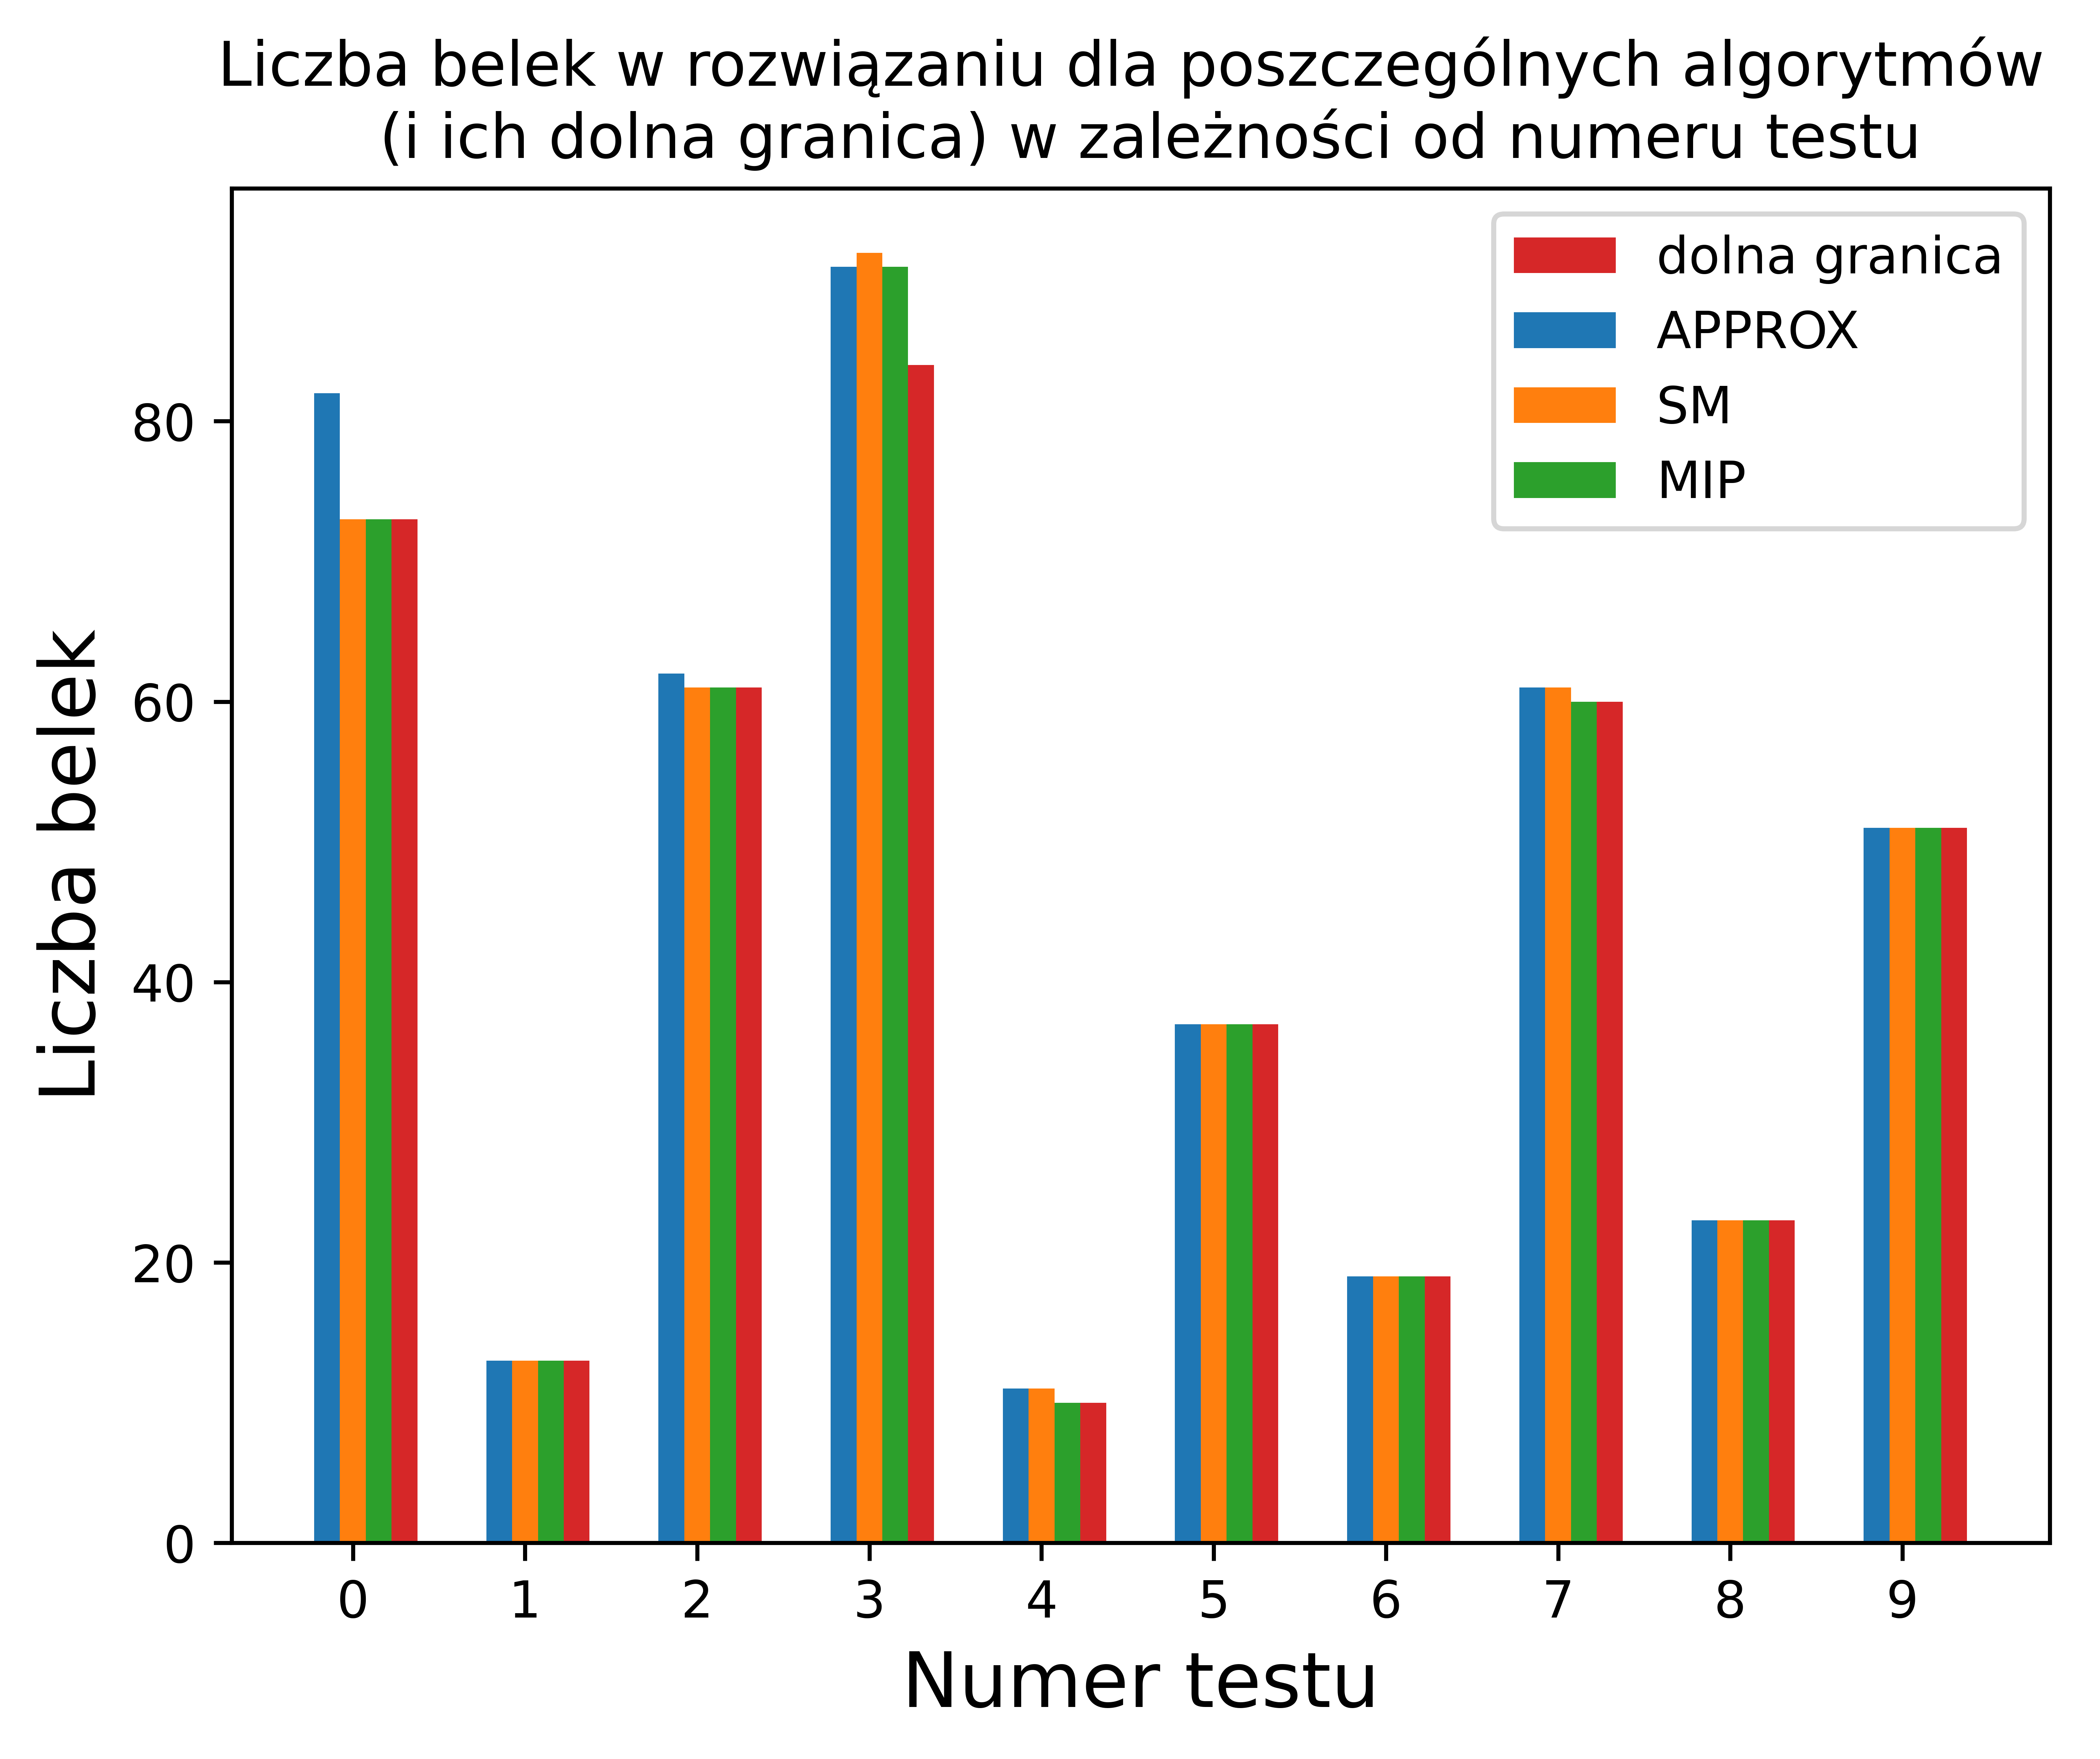
\includegraphics[width=12cm]{plots/res}
	\caption{Wykres przedstawiający liczbę belek (i ich dolną granicę) w rozwiązaniu dla poszczególnych algorytmów w zależności od numeru testu.}
	\end{center}
\end{figure}

\begin{figure}[H]
	\begin{center}
		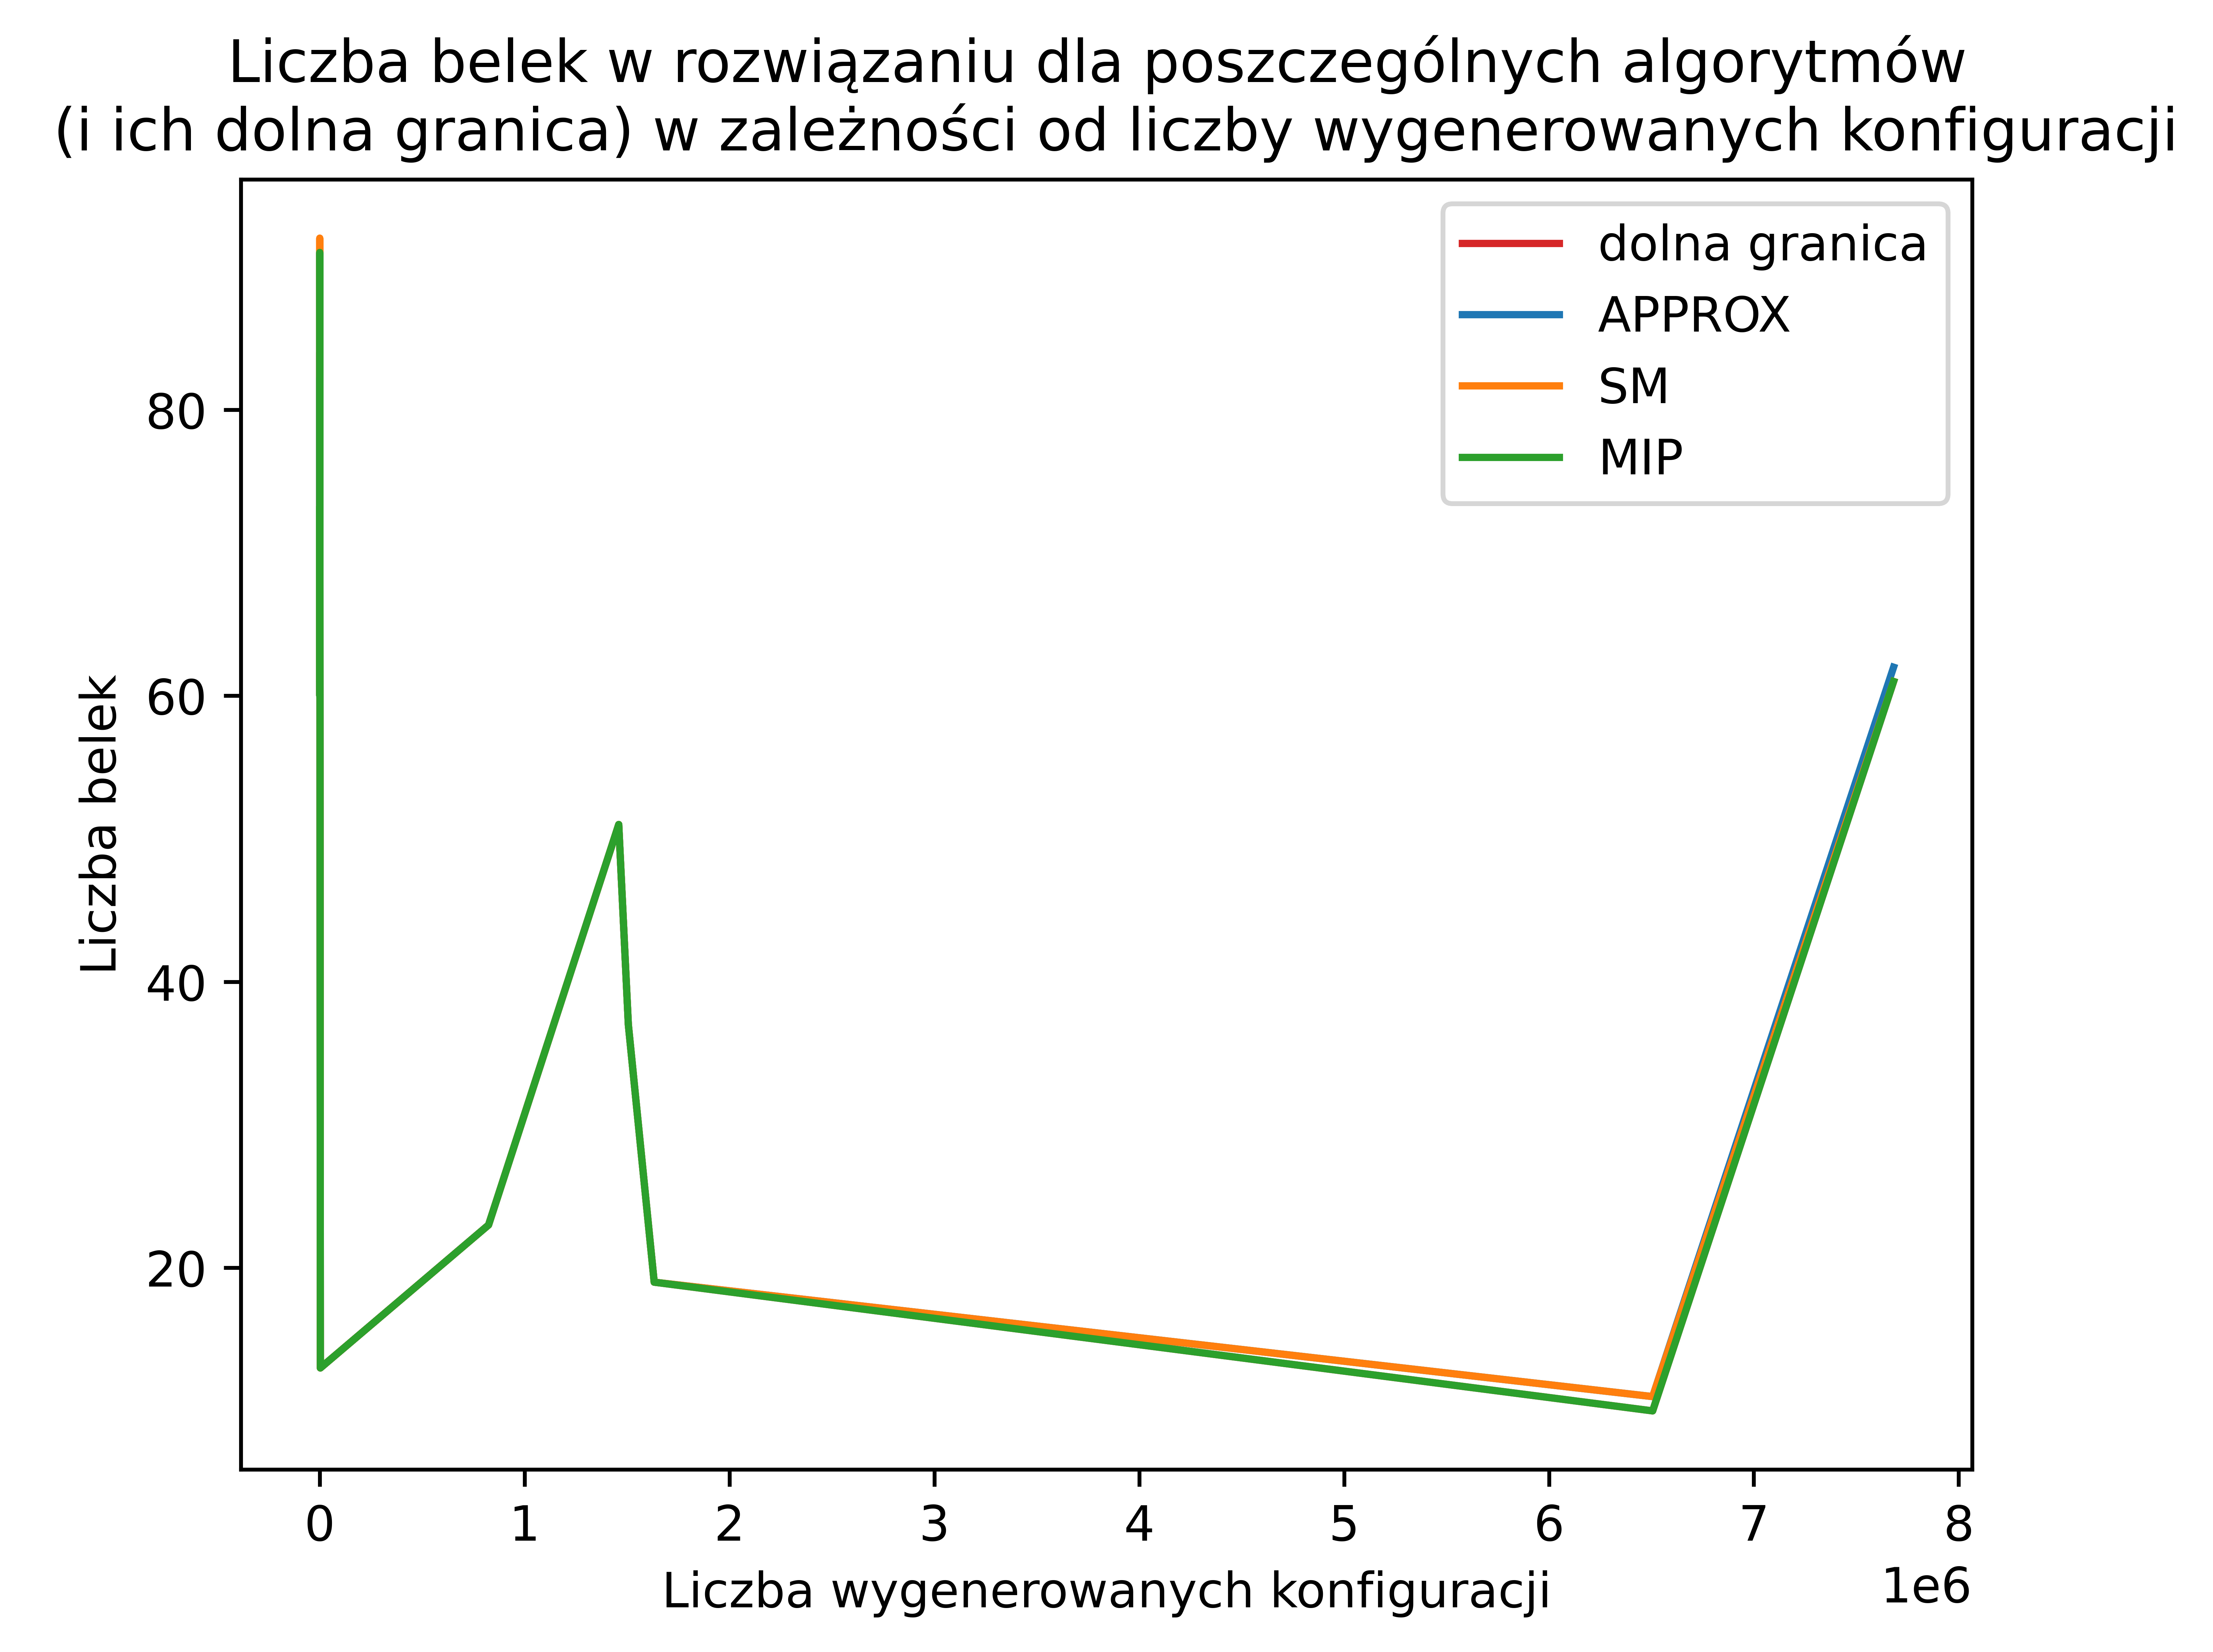
\includegraphics[width=12cm]{plots/res_configs}
		\caption{Wykres przedstawiający liczbę belek (i ich dolną granicę) w rozwiązaniu dla poszczególnych algorytmów w zależności od liczby wygenerowanych konfiguracji.}
	\end{center}
\end{figure}

\subsection{Czas wykonania}

\begin{table}[H] 
	\begin{center}
		\begin{tabular}{|p{3cm}|p{3cm}|p{3cm}|p{3cm}| } \hline
			Numer testu & APPROX & SM & MIP\\ \hline
			0 & 0.001 & 0.002 & 0.006\\ 
			1 & 0.001 & 0.004 & 0.055\\ 
			2 & 0.002 & 180.953 & 10076.226\\ 
			3 & 0.001 & 0.002 & 0.003\\ 
			4 & 0.001 & 7.963 & 1398.353\\ 
			5 & 0.002 & 4.625 & 1211.544\\ 
			6 & 0.001 & 4.218 & 779.089\\ 
			7 & 0.001 & 0.002 & 0.017\\ 
			8 & 0.001 & 1.720 & 434.735\\ 
			
			\hline
		\end{tabular}
		\caption{Czas wykonania progamu (w sekundach) dla poszczególnych algorytmów i testów}
	\end{center}
\end{table}

\begin{figure}[H]
	\begin{center}
		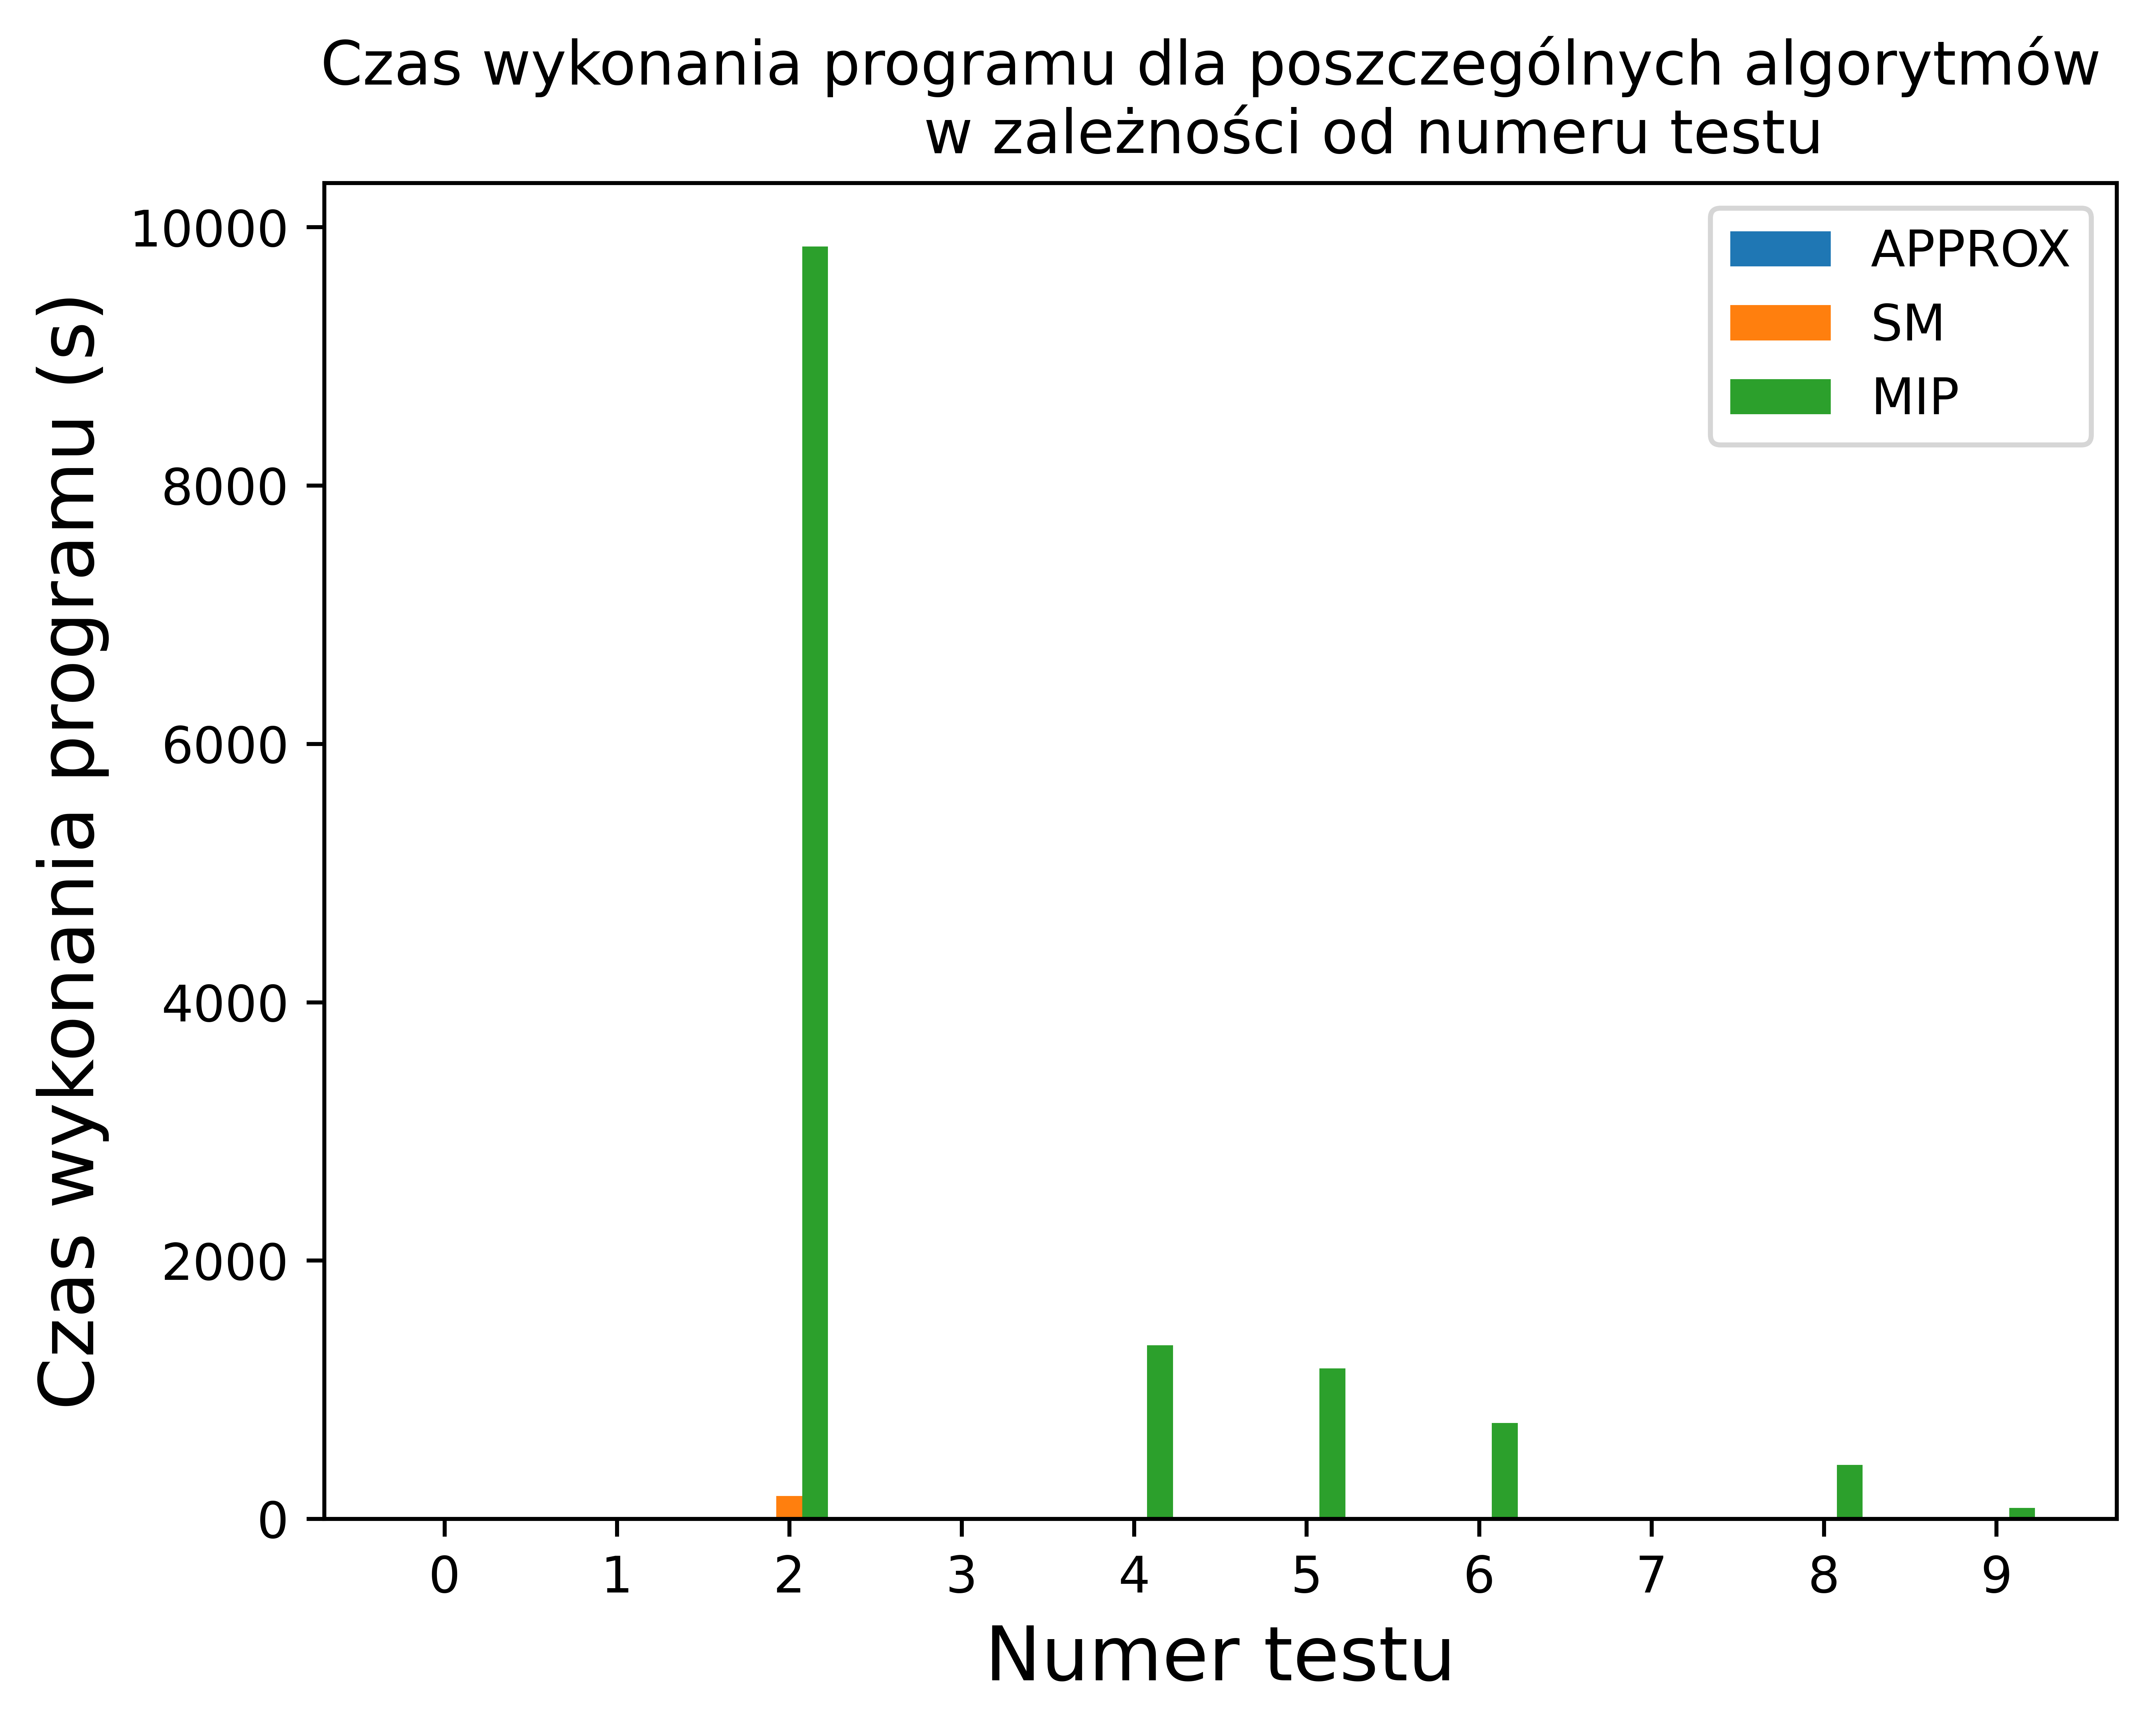
\includegraphics[width=12cm]{plots/time}
		\caption{Wykres przedstawiający czas wykonania programu dla poszczególnych algorytmów w zależności od numeru testu.}
	\end{center}
\end{figure}

\begin{figure}[H]
	\begin{center}
		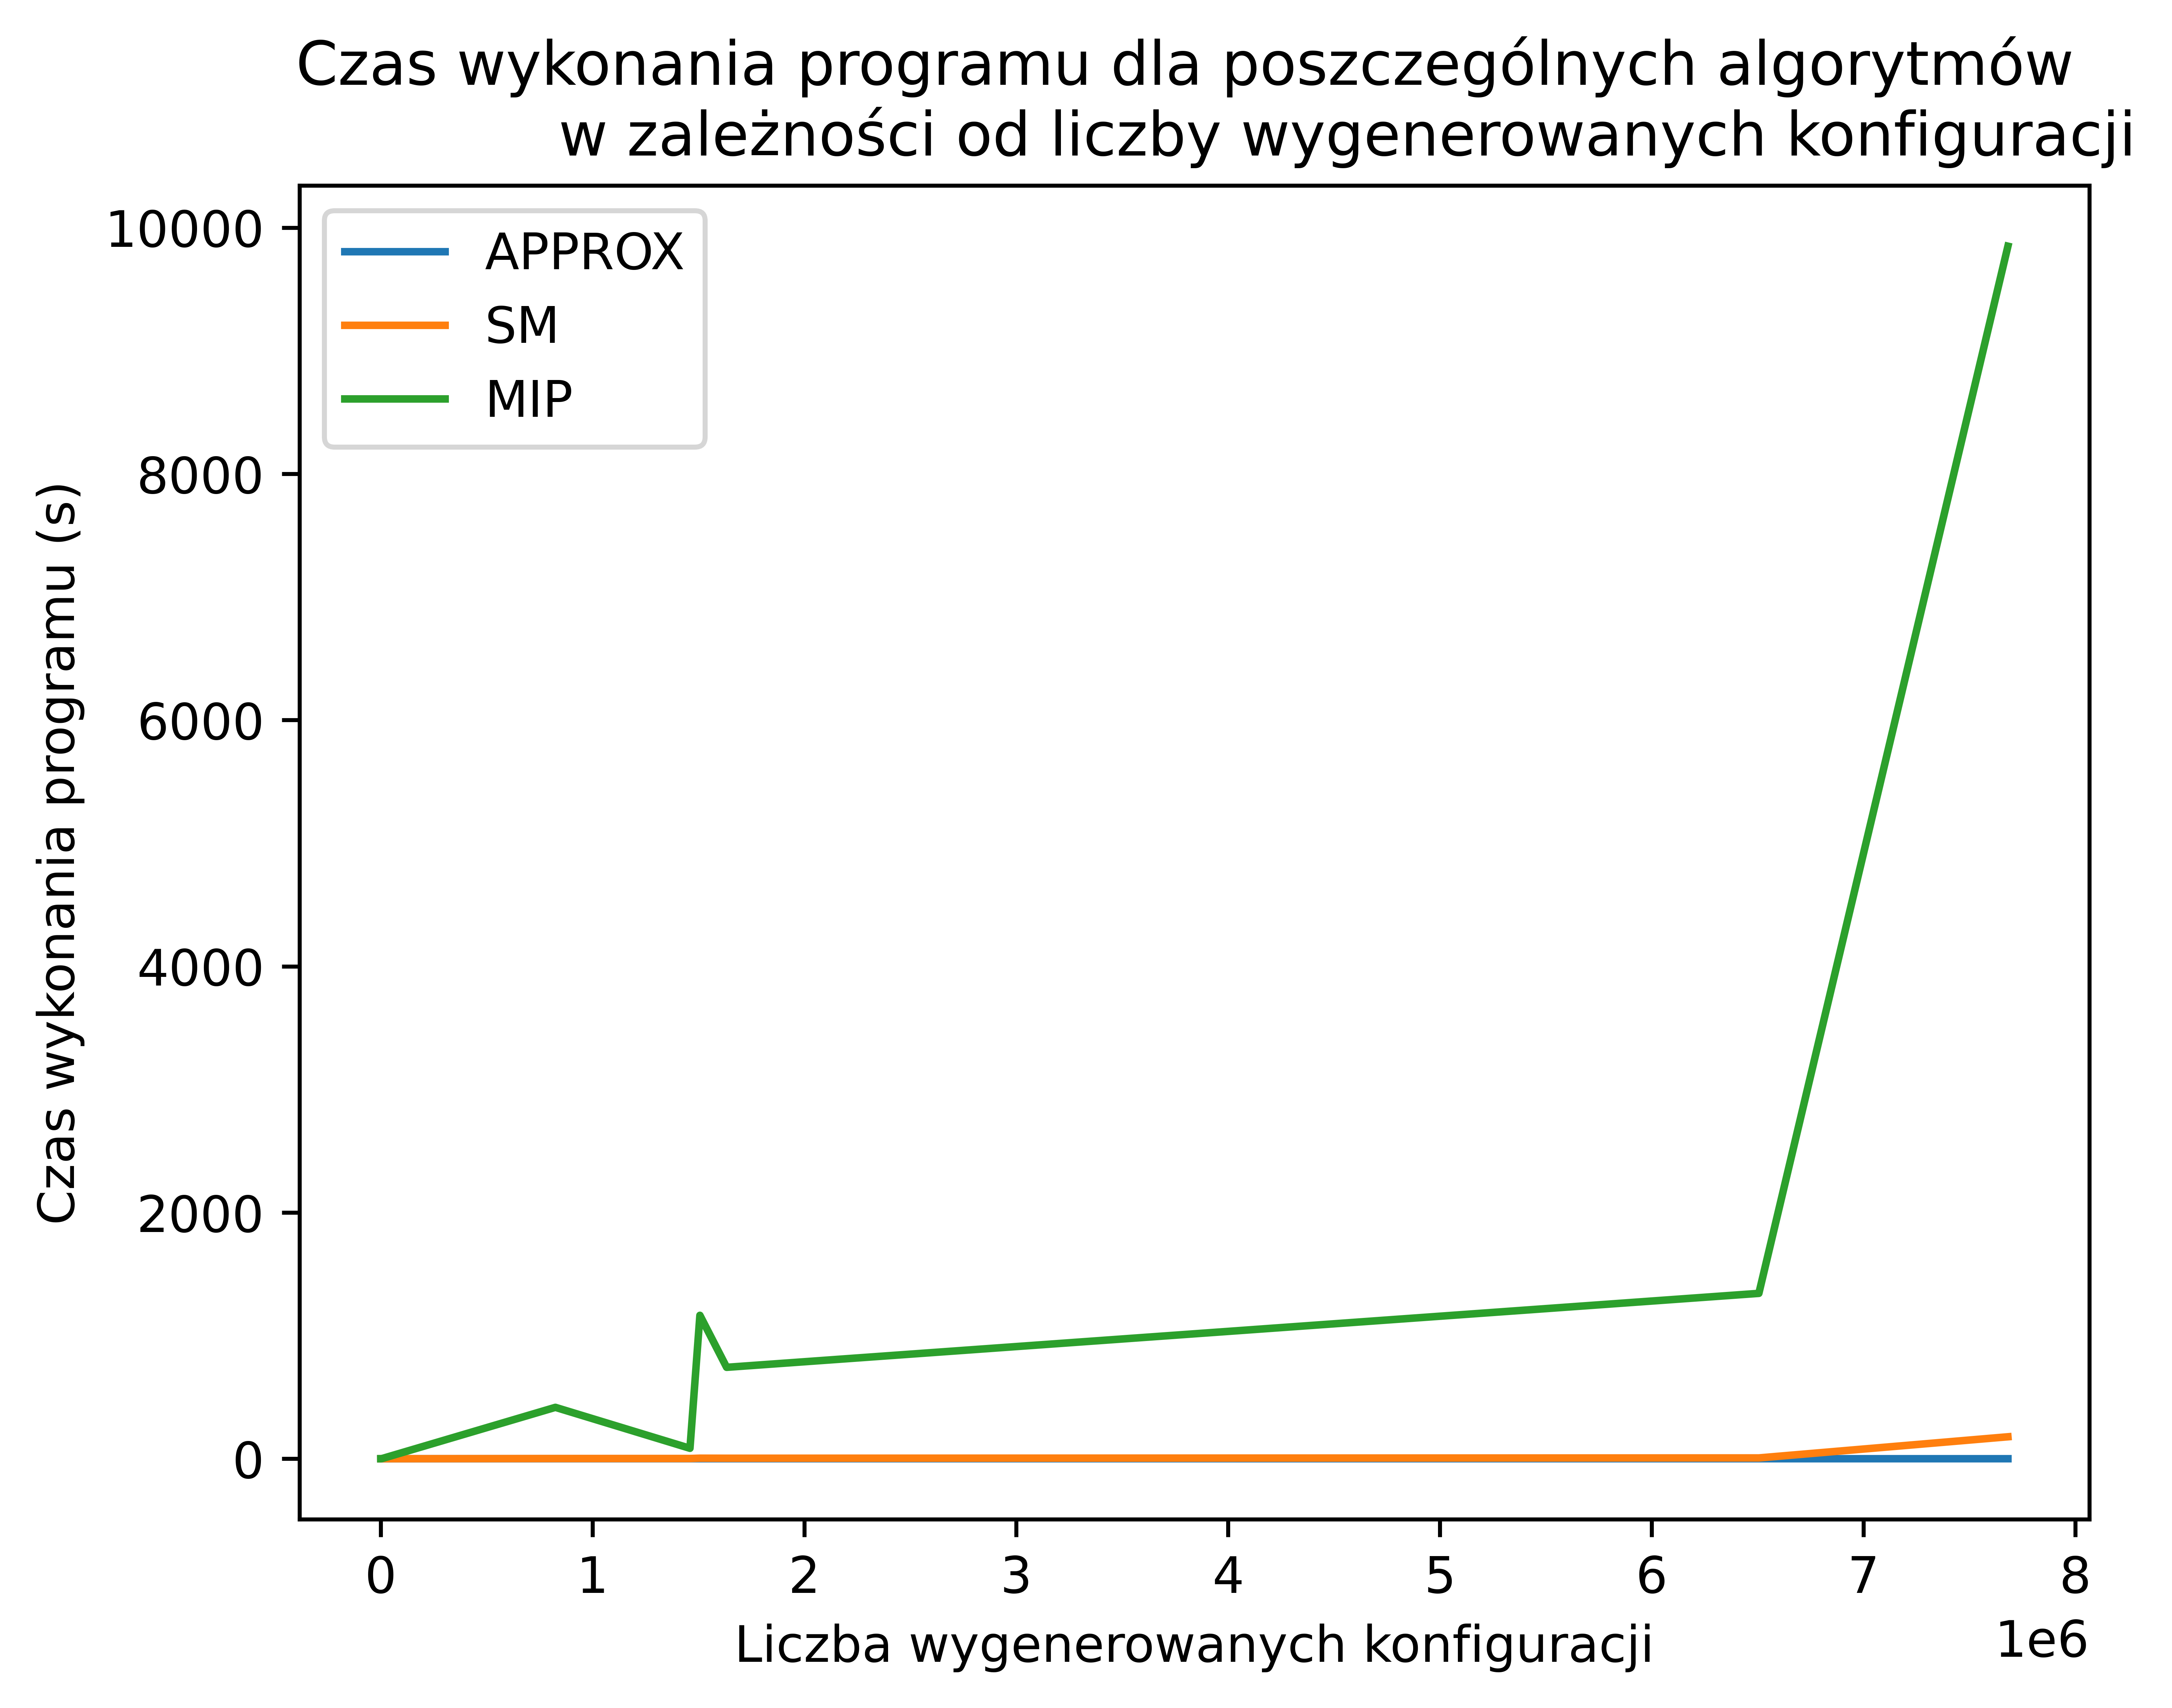
\includegraphics[width=12cm]{plots/time_configs}
		\caption{Wykres przedstawiający czas wykonania programu dla poszczególnych algorytmów w zależności od liczby wygenerowanych konfiguracji.}
	\end{center}
\end{figure}


\section{Wnioski}
Pierwszym co można zauważyć z zaprezentowanych powyżej danych jest to, że otrzymane rozwiązania są często blisko dolnej granicy. Jedynie w teście o numerze zero różnica ta wynosi aż dziewięc belek dla algorytmu aproksymacyjnego. Policzmy czy mieście się to we współczynniku aproksymacji: $73*11/9=89,(2) \leq 83$. Odpowiedź jest twierdząca. 
Drugią kwestią jest bardzo zróźnicowany czas działana algorytmów.
Program używający algolrytmu aproksymacyjnego nie przekroczył nigdy dwóch milisekund. Natomiast MIP potrafił działać nawet prawie 3h (test drugi - 10076.226s) zanim znalazł optymalne rozwiązanie. Jednak to nie sama optymalizacja liniowa powoduje taki narzut czasu. Gdy popatrzymy w teście piątym na algorytm SM, czas jego wykonywania jest prawie 261 razy krótszy ($1211.544÷4.625 \approx 261,95$). Nasuwa się tu wniosek, że to znalezienie rozwiązania optymalnego pod kątem całkowitoliczbowym jest za to odpowiedzialne (sekwencja branch-and-cut następująca po optymalizacji sympleksowej). 
Pierwszym wytłumaczeniem tego może być informacja zawarta w dokumentacji GLPK: \textit{GLPK branch-and-cut solver is not perfect, so it is unable to solve hard or very large scale MIP instances for a reasonable time.} 
Jednakże można zastanowić się czy algorytm approksymacyjny nie zwraca zadowalających wyników, skoro w powyższych testach tylko cztery razy był gorszy od MIP (w tym trzy razy różnica wynosiła jedną belkę). Gdyby jednak zależało nam na obsłużeniu skrajnych przypadków, SM radzi sobie w nich lepiej od samego aproksymacyjnego, podobnie do MIP, ale za to często w łatwych przykładach jest gorszy od tego pierwszego.




	\cleardoublepage
	
	\chapter{Testy}  
\thispagestyle{chapterBeginStyle}
\label{ch:CHAPTER_4}

\section{Informacje wstępne}
Zbiór danych na których zostały przeprowadzone testy znajduje się w katalogu \verb|Tests/input|. Każdy z dziesięciu plików, których nazwy trzymają się konwencji: test$<$numer\_testu$>$.txt, jest zgodny z formatem opisanym w sekcji \ref{format_danych}, gdzie $<$numer\_testu$>$ to liczba naturalna ze zbioru $\{0, ..., 9\}$.

Do pomiaru czasu wykonania zostało wykorzystane linuksowe polecenie \textbf{time} - brana pod uwagę była tylko ilość czasu procesora spędzonego w trybie użytkownika. Pominięty został czas spędzony w jądrze systemu - czytanie wejścia, alokacje pamięci.

Za automatyzację uruchamiania programu na poszczególnych plikach i algorytmach odpowiada skrypt napisany w języku powłoki bash - plik \verb|Tests/run_tests.sh|. Iteruje on po plikach z katalogu w którym znajduja się dane testowe, po algorytmach, wyznacza nazwy plików według określonego schematu i wywołuje komendę: \\
\verb|{ time $EXEC_FILE -f $infile -o $resultfilename -a $algo > $solver_log ;} 2> $time_filename|, 

\begin{itemize}
	\item \$EXEC\_FILE - ścieżka do skompilowanego programu
	\item \$infile - plik z danymi wejściowymi: \\
	\verb|Tests/input/test<numer_testu>.txt|
	\item \$resultfilename - ścieżka do pliku z rozwiązaniem: \\ \verb|Tests/output/test<numer_testu>_<algorytm>_res.txt| (patrz rysunek \ref{output_example})
	\item \$algo - algorytm (APPROX, MIP, SM)
	\item \$solver\_log - ścieżka do pliku w którym zostanie zapisane standardowe wyjście programu, a na które drukuje bibliotek GLPK podczas optymalizacji
	\item \$time\_filename - ścieżka do pliku z rezulatatem polecenia \textbf{time}
\end{itemize}

Wykresy i tabele wyegenrowane zostały za pomocą skryptu pythonowego: \\ \verb|Tests/generate_plots.py|.

Oznaczenia:
\begin{itemize}
	\item APPROX - program używał algorytmu aproksymacyjnego
	\item MIP - program używał solvera MIP (branch and cut)
	\item SM - program używał solver simpleksowego i zaokrąglał wyniki algorytmem aproksymacyjnym
\end{itemize}

Platforma testowa to komputer stacjonarny z czterordzeniowym procesorem Intel Core i5-3570K, 16GB pamięci RAM DDR3 CL9.

Warto dodać, że test numer dwa pochodzi od EURO Special Interest Group on Cutting and Packings. Dane testowe przez nich dostarczone można znaleźć pod tym linkiem:
\href{https://www.euro-online.org/websites/esicup/data-sets/}{ESICUP dataset}.
Konkretnie jest to pozycja \textit{The 28 VERY hard BPP instances of J. Schoenfield (with m from 140 to 200). Test results with an LP-based approach in (Data sets: hard28)} - próba o nazwie \textit{'BPP    14'}. Zawiera on podobny format danych opisanych wcześniej z tą różnicą, że długośc belki i liczba elementów są zamienione wierszami. Jednakże testowany w tej pracy przykład rozpatruje najmniejszy element długości 40 - stąd liczba typów 126 zamiast pierwotnych 136. Spowodowane było to problemem z wykorzystaniem całej dostępnej pamięci operacyjnej platformy testowej dla drugiej wartości. Owe dane testowe łamią też w pewnym sensie koncepcję przyjęcia za liczbę typów stałej. Największa liczba elementów danego typu jaka występuje to 2, zazwyczaj wynosi ona jeden, więc pomimo liczby typów wynoszącej 126, wszystkich elementów jest 148. Same instancje problemów zostały określone jako \textit{bardzo trudne}.



\begin{table}[H] 
	\begin{center}
		\begin{tabular}{|p{3cm}|p{3cm}|p{3cm}|p{3cm}|p{3cm}| } \hline
			Numer testu & Długość belki & Liczba typów elementów & Liczba wszystkich elementów ($n$) & Liczba wygenerowanych konfiguracji\\ 
			\hline
			0 & 5600 & 13 & 219 & 213\\ 
			1 & 1200 & 4 & 343 & 3563\\ 
			2 & 1000 & 126 & 148 & 7682204\\ 
			3 & 600 & 10 & 225 & 636\\ 
			4 & 6000 & 12 & 178 & 6506312\\ 
			5 & 4500 & 18 & 190 & 1506800\\ 
			6 & 7300 & 12 & 130 & 1632979\\ 
			7 & 120 & 10 & 227 & 614\\ 
			8 & 3000 & 15 & 187 & 824526\\ 
			9 & 1000 & 12 & 394 & 1459890\\ 
			
			\hline
		\end{tabular}
		\caption{Podstawowe dadne dotyczące poszczególnych testów.}
	\end{center}
\end{table}


\section{Wyniki}

Dla każdego testu solver był w stanie znaleźć rozwiązanie i zwrócił komunikaty:
\begin{itemize}
	\item ``OPTIMAL LP SOLUTION FOUND`` dla metody simpleksowej
	\item ``INTEGER OPTIMAL SOLUTION FOUND`` dla metody MIP
\end{itemize}

\subsection{Liczba belek}

%\iffalse

\begin{table}[H] 
	\begin{center}
	\begin{tabular}{|p{3cm}|p{3cm}|p{3cm}|p{3cm}|p{3cm}| } 
		\hline
			Numer testu & APPROX & SM & MIP & Dolna granica\\ 
			\hline
			0 & 82 & 73 & 73 & 73\\ 
			1 & 13 & 13 & 13 & 13\\ 
			2 & 62 & 61 & 61 & 61\\ 
			3 & 91 & 92 & 91 & 84\\ 
			4 & 11 & 11 & 10 & 10\\ 
			5 & 37 & 37 & 37 & 37\\ 
			6 & 19 & 19 & 19 & 19\\ 
			7 & 61 & 61 & 60 & 60\\ 
			8 & 23 & 23 & 23 & 23\\ 
			9 & 51 & 51 & 51 & 51\\ 
			\hline
		\end{tabular}
			\caption{Liczba belek dla poszczególnych algorytmów w zależności od numeru testu.}
	\end{center}
\end{table}

\begin{figure}[H]
	\begin{center}
	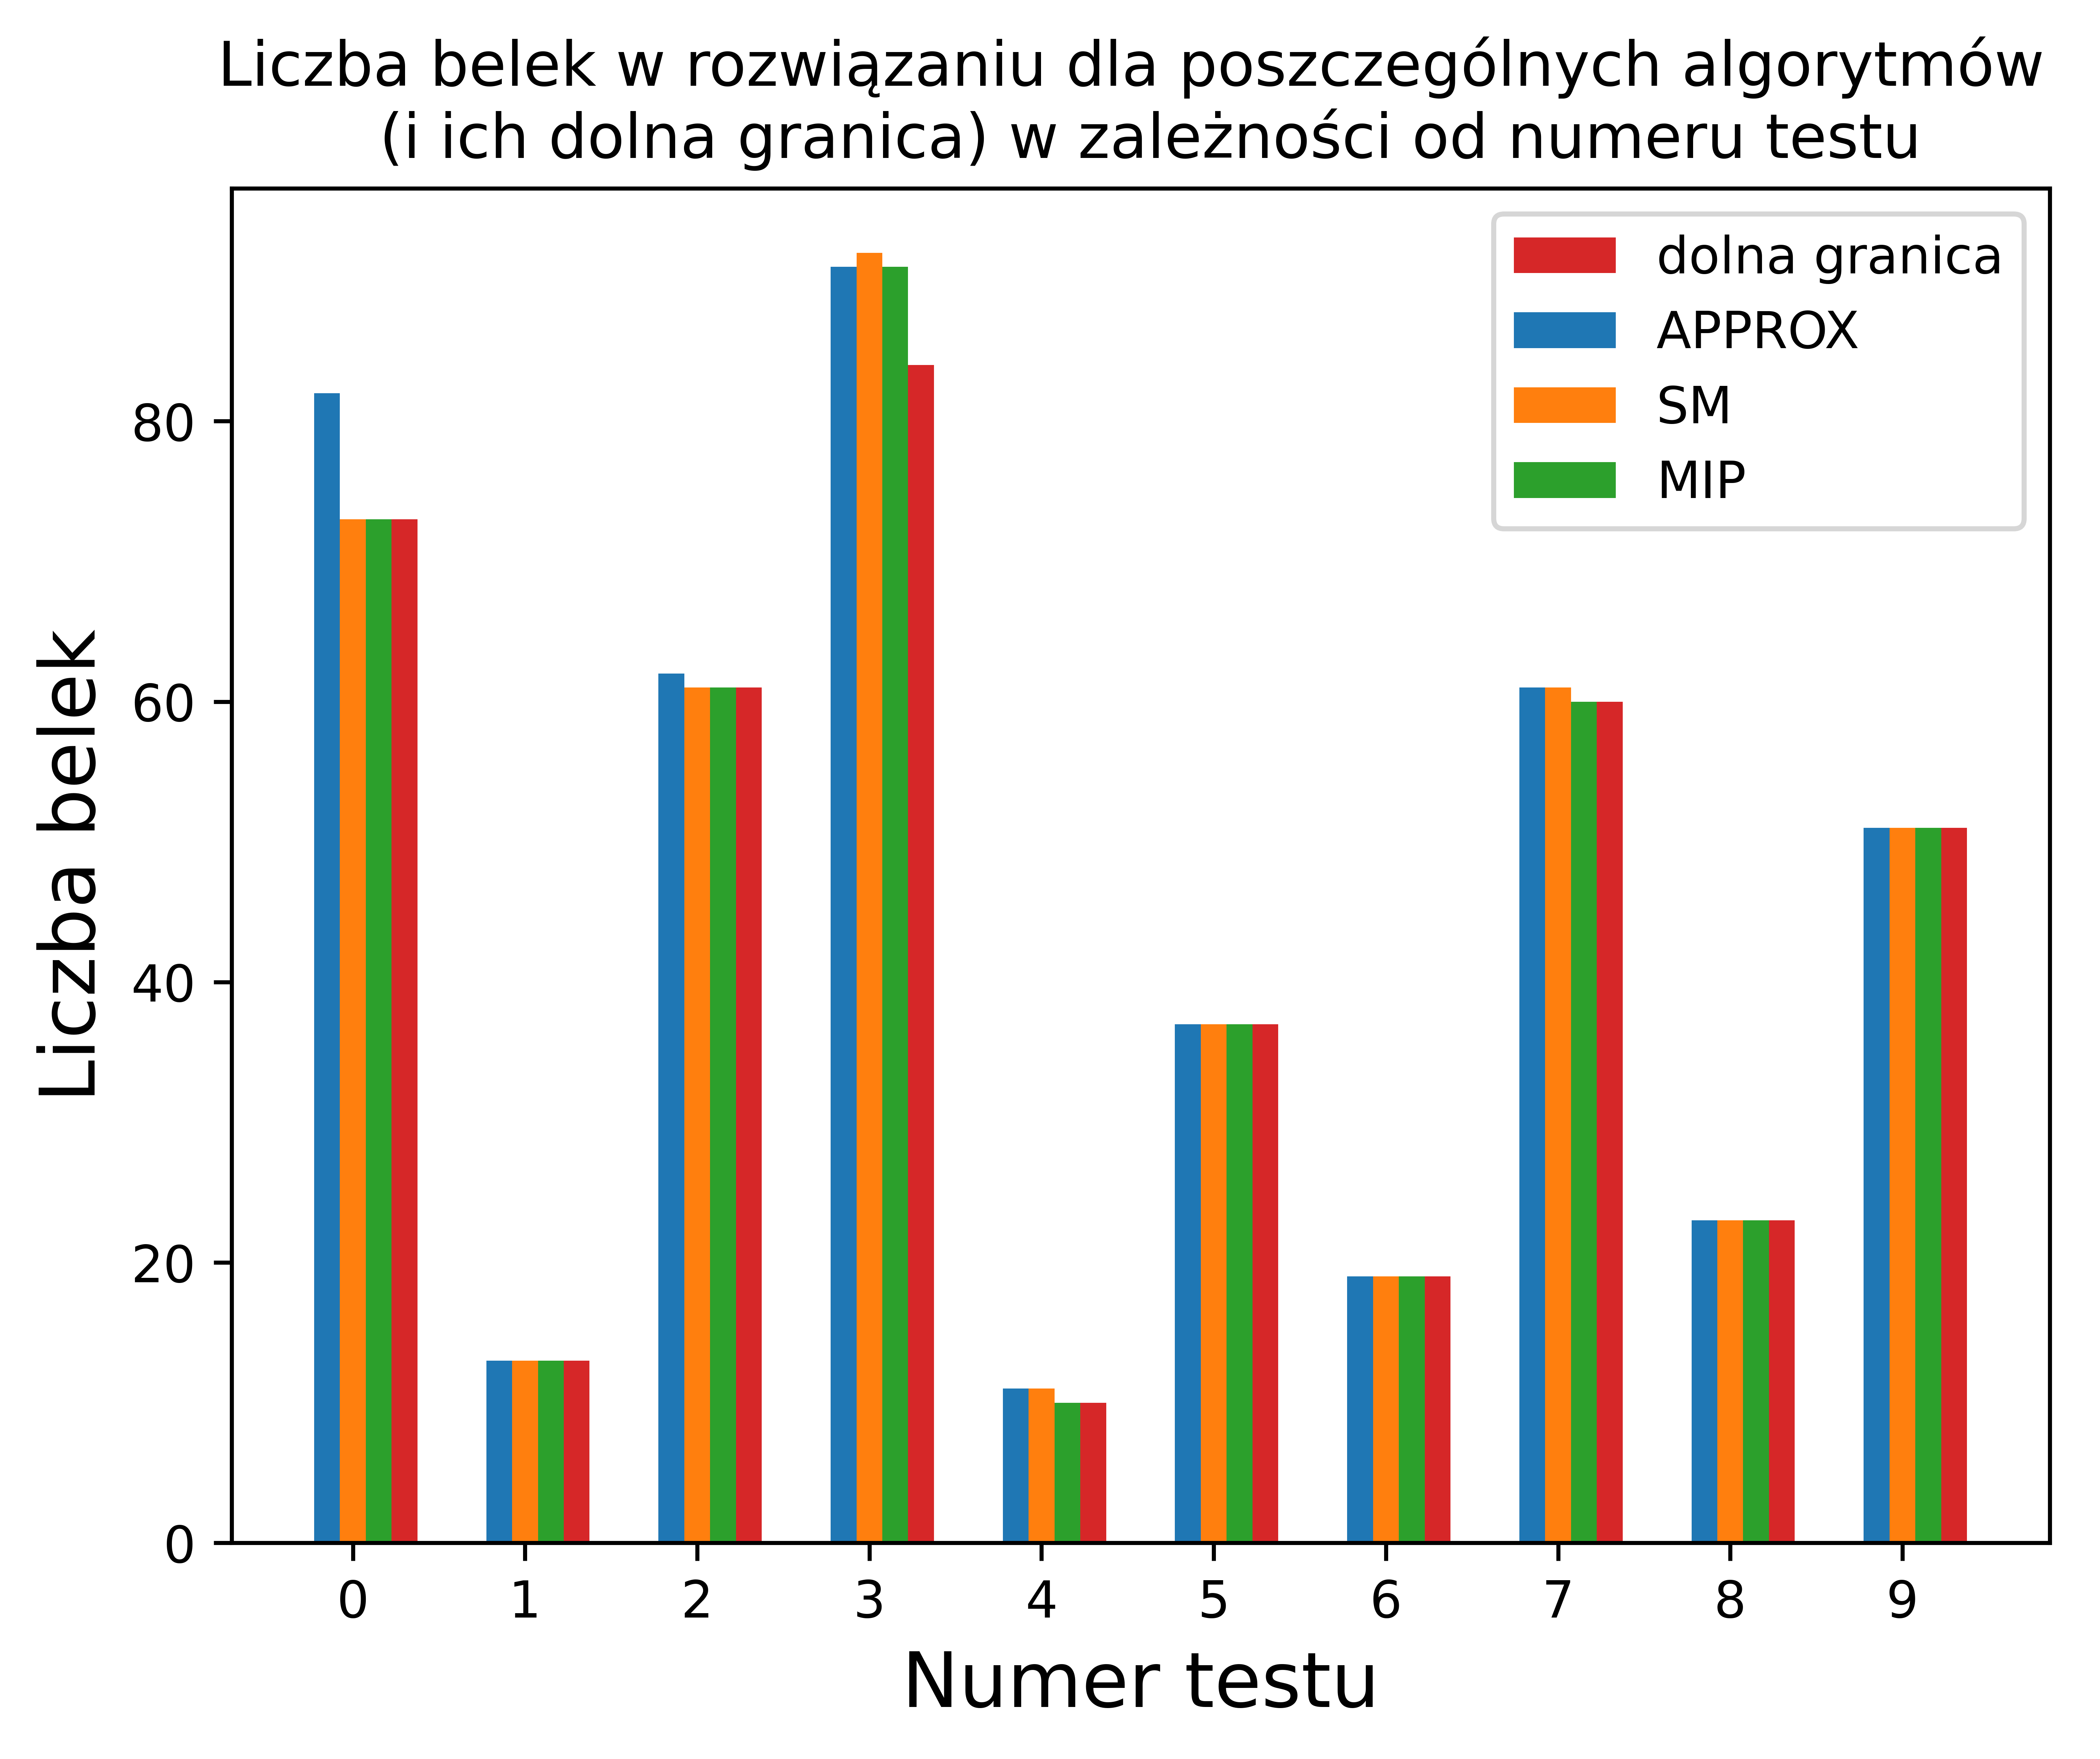
\includegraphics[width=12cm]{plots/res}
	\caption{Wykres przedstawiający liczbę belek (i ich dolną granicę) w rozwiązaniu dla poszczególnych algorytmów w zależności od numeru testu.}
	\end{center}
\end{figure}

\begin{figure}[H]
	\begin{center}
		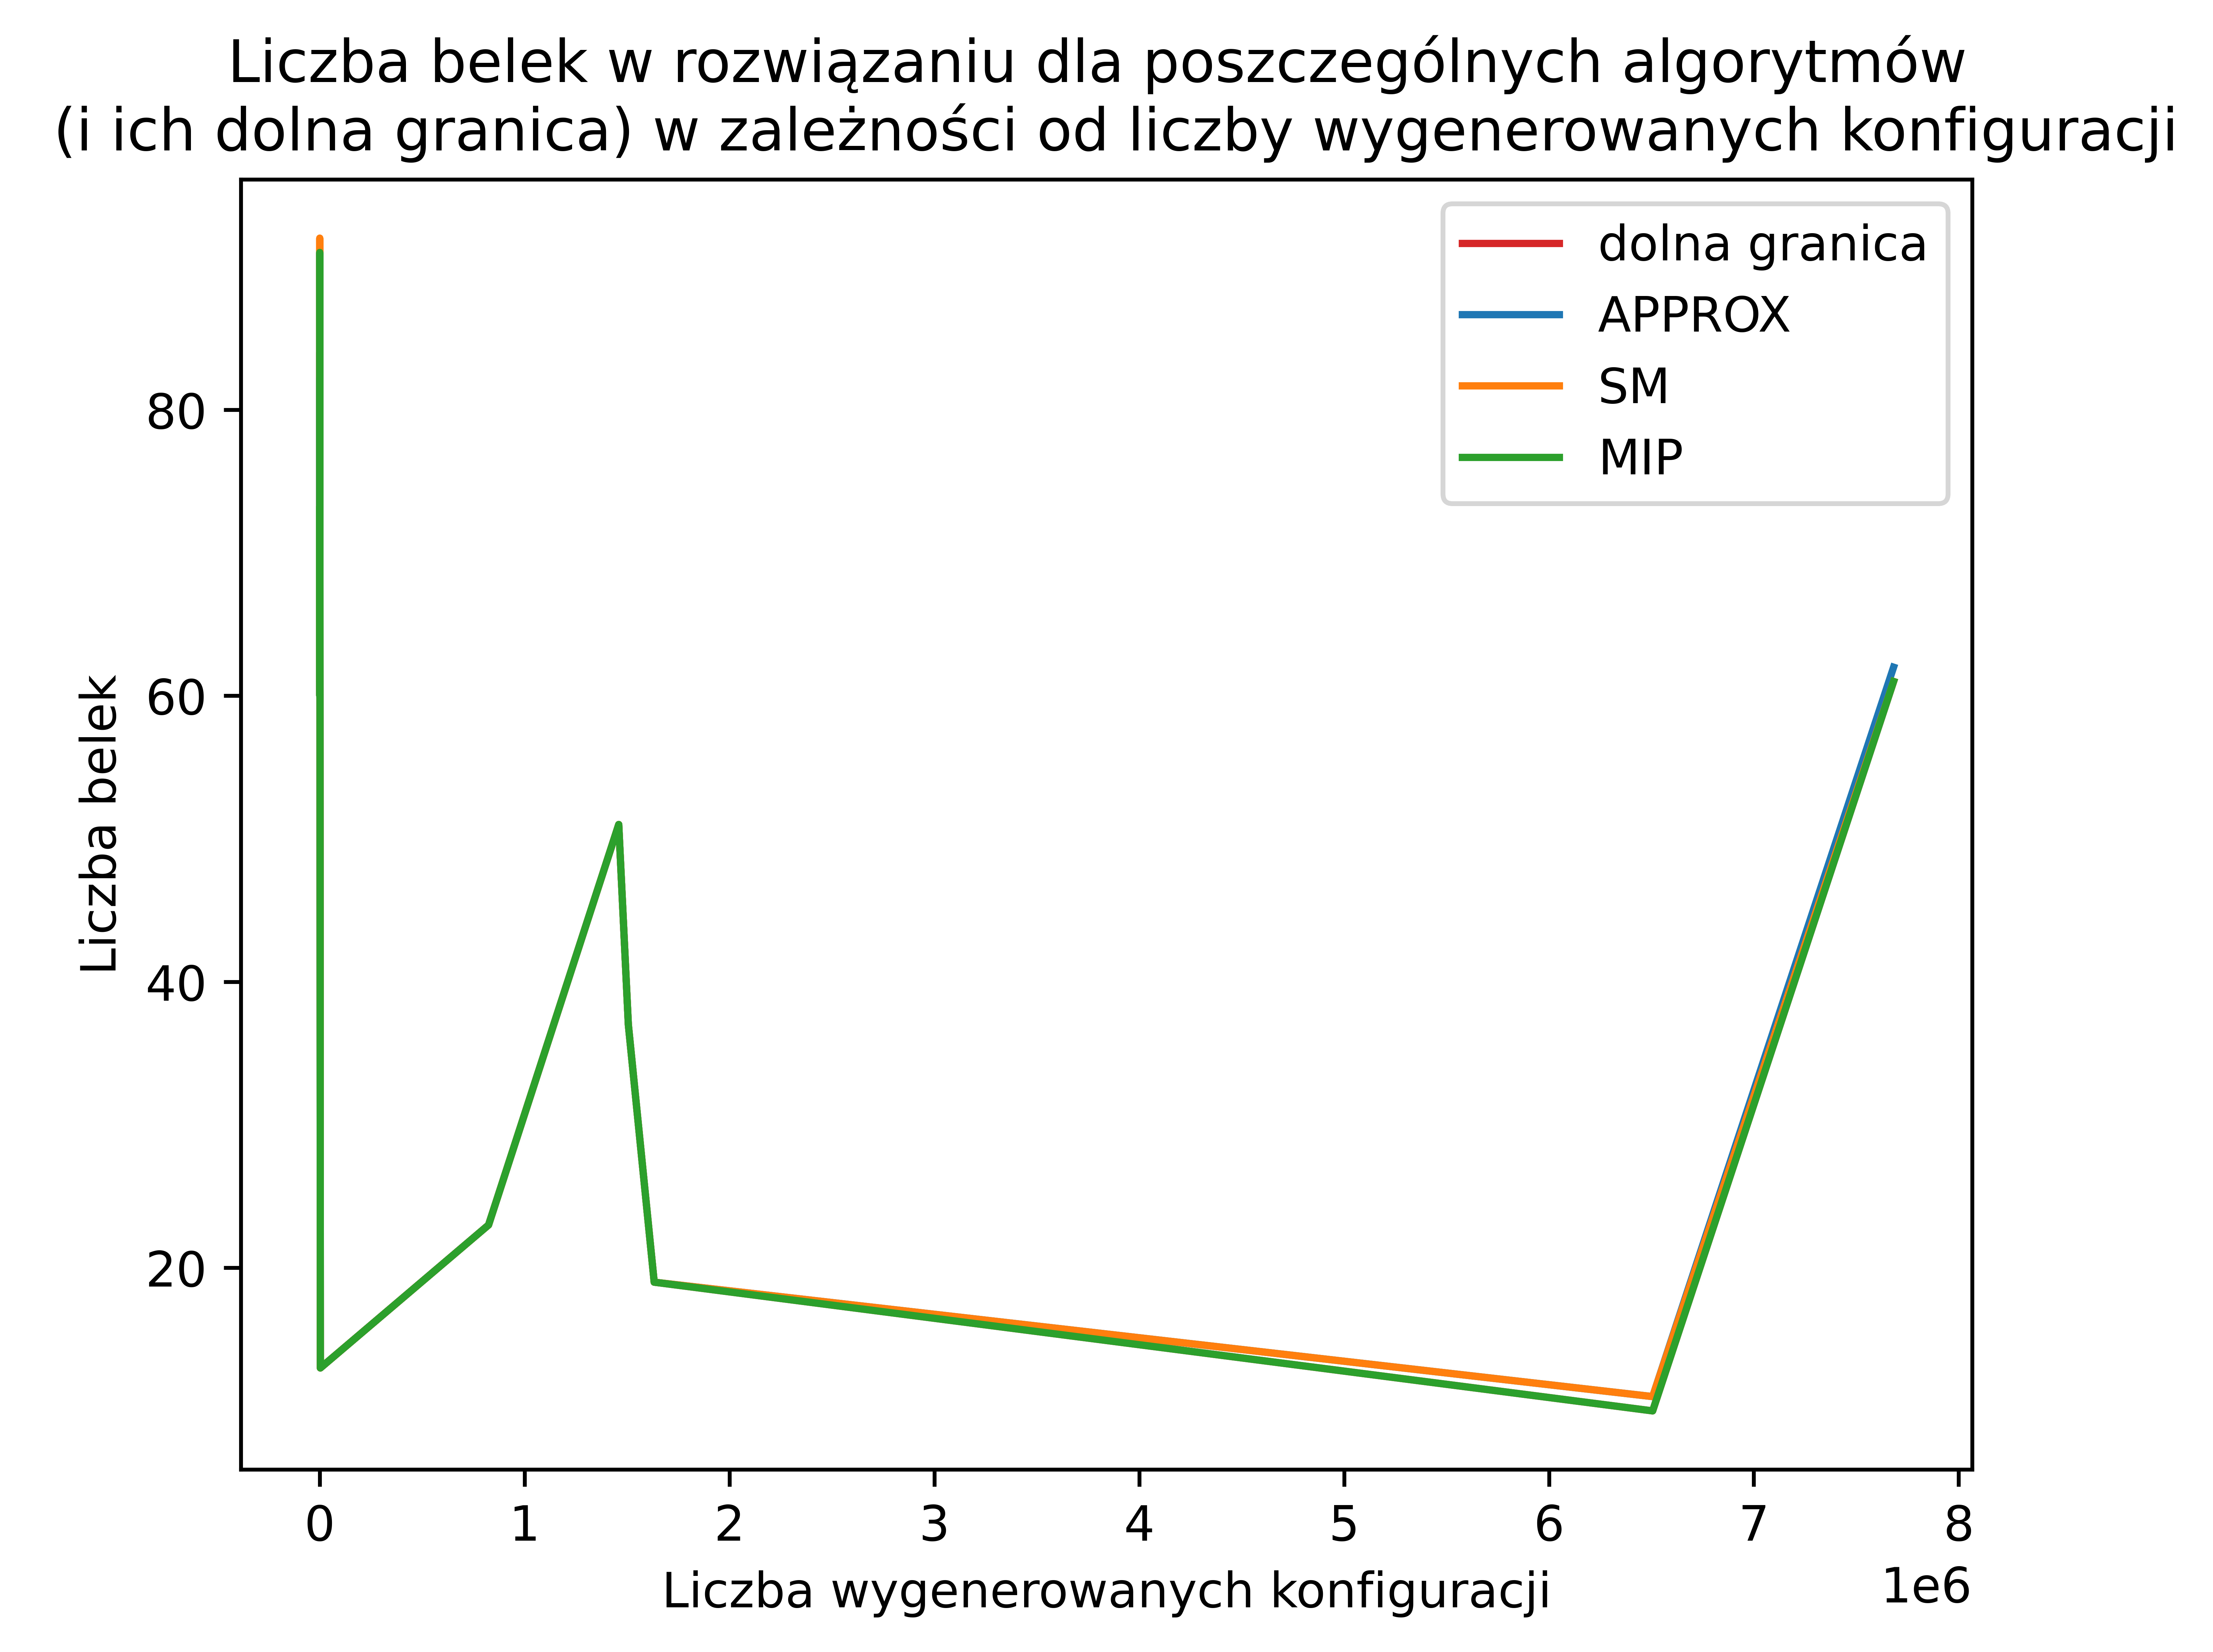
\includegraphics[width=12cm]{plots/res_configs}
		\caption{Wykres przedstawiający liczbę belek (i ich dolną granicę) w rozwiązaniu dla poszczególnych algorytmów w zależności od liczby wygenerowanych konfiguracji.}
	\end{center}
\end{figure}

\subsection{Czas wykonania}


\begin{table}[H] 
	\begin{center}
		\begin{tabular}{|p{3cm}|p{3cm}|p{3cm}|p{3cm}| } \hline
			Numer testu & APPROX & SM & MIP\\ 
			\hline
			0 & 0.001 & 0.002 & 0.006\\ 
			1 & 0.001 & 0.000 & 0.050\\ 
			2 & 0.002 & 178.151 & 9849.150\\ 
			3 & 0.001 & 0.000 & 0.003\\ 
			4 & 0.001 & 6.527 & 1343.093\\ 
			5 & 0.000 & 4.271 & 1164.734\\ 
			6 & 0.001 & 3.837 & 742.420\\ 
			7 & 0.000 & 0.002 & 0.017\\ 
			8 & 0.001 & 1.533 & 417.277\\ 
			9 & 0.001 & 1.804 & 84.618\\ 
			\hline
		\end{tabular}
		\caption{Czas wykonania progamu (w sekundach) dla poszczególnych algorytmów i testów.}
	\end{center}
\end{table}

\begin{figure}[H]
	\begin{center}
		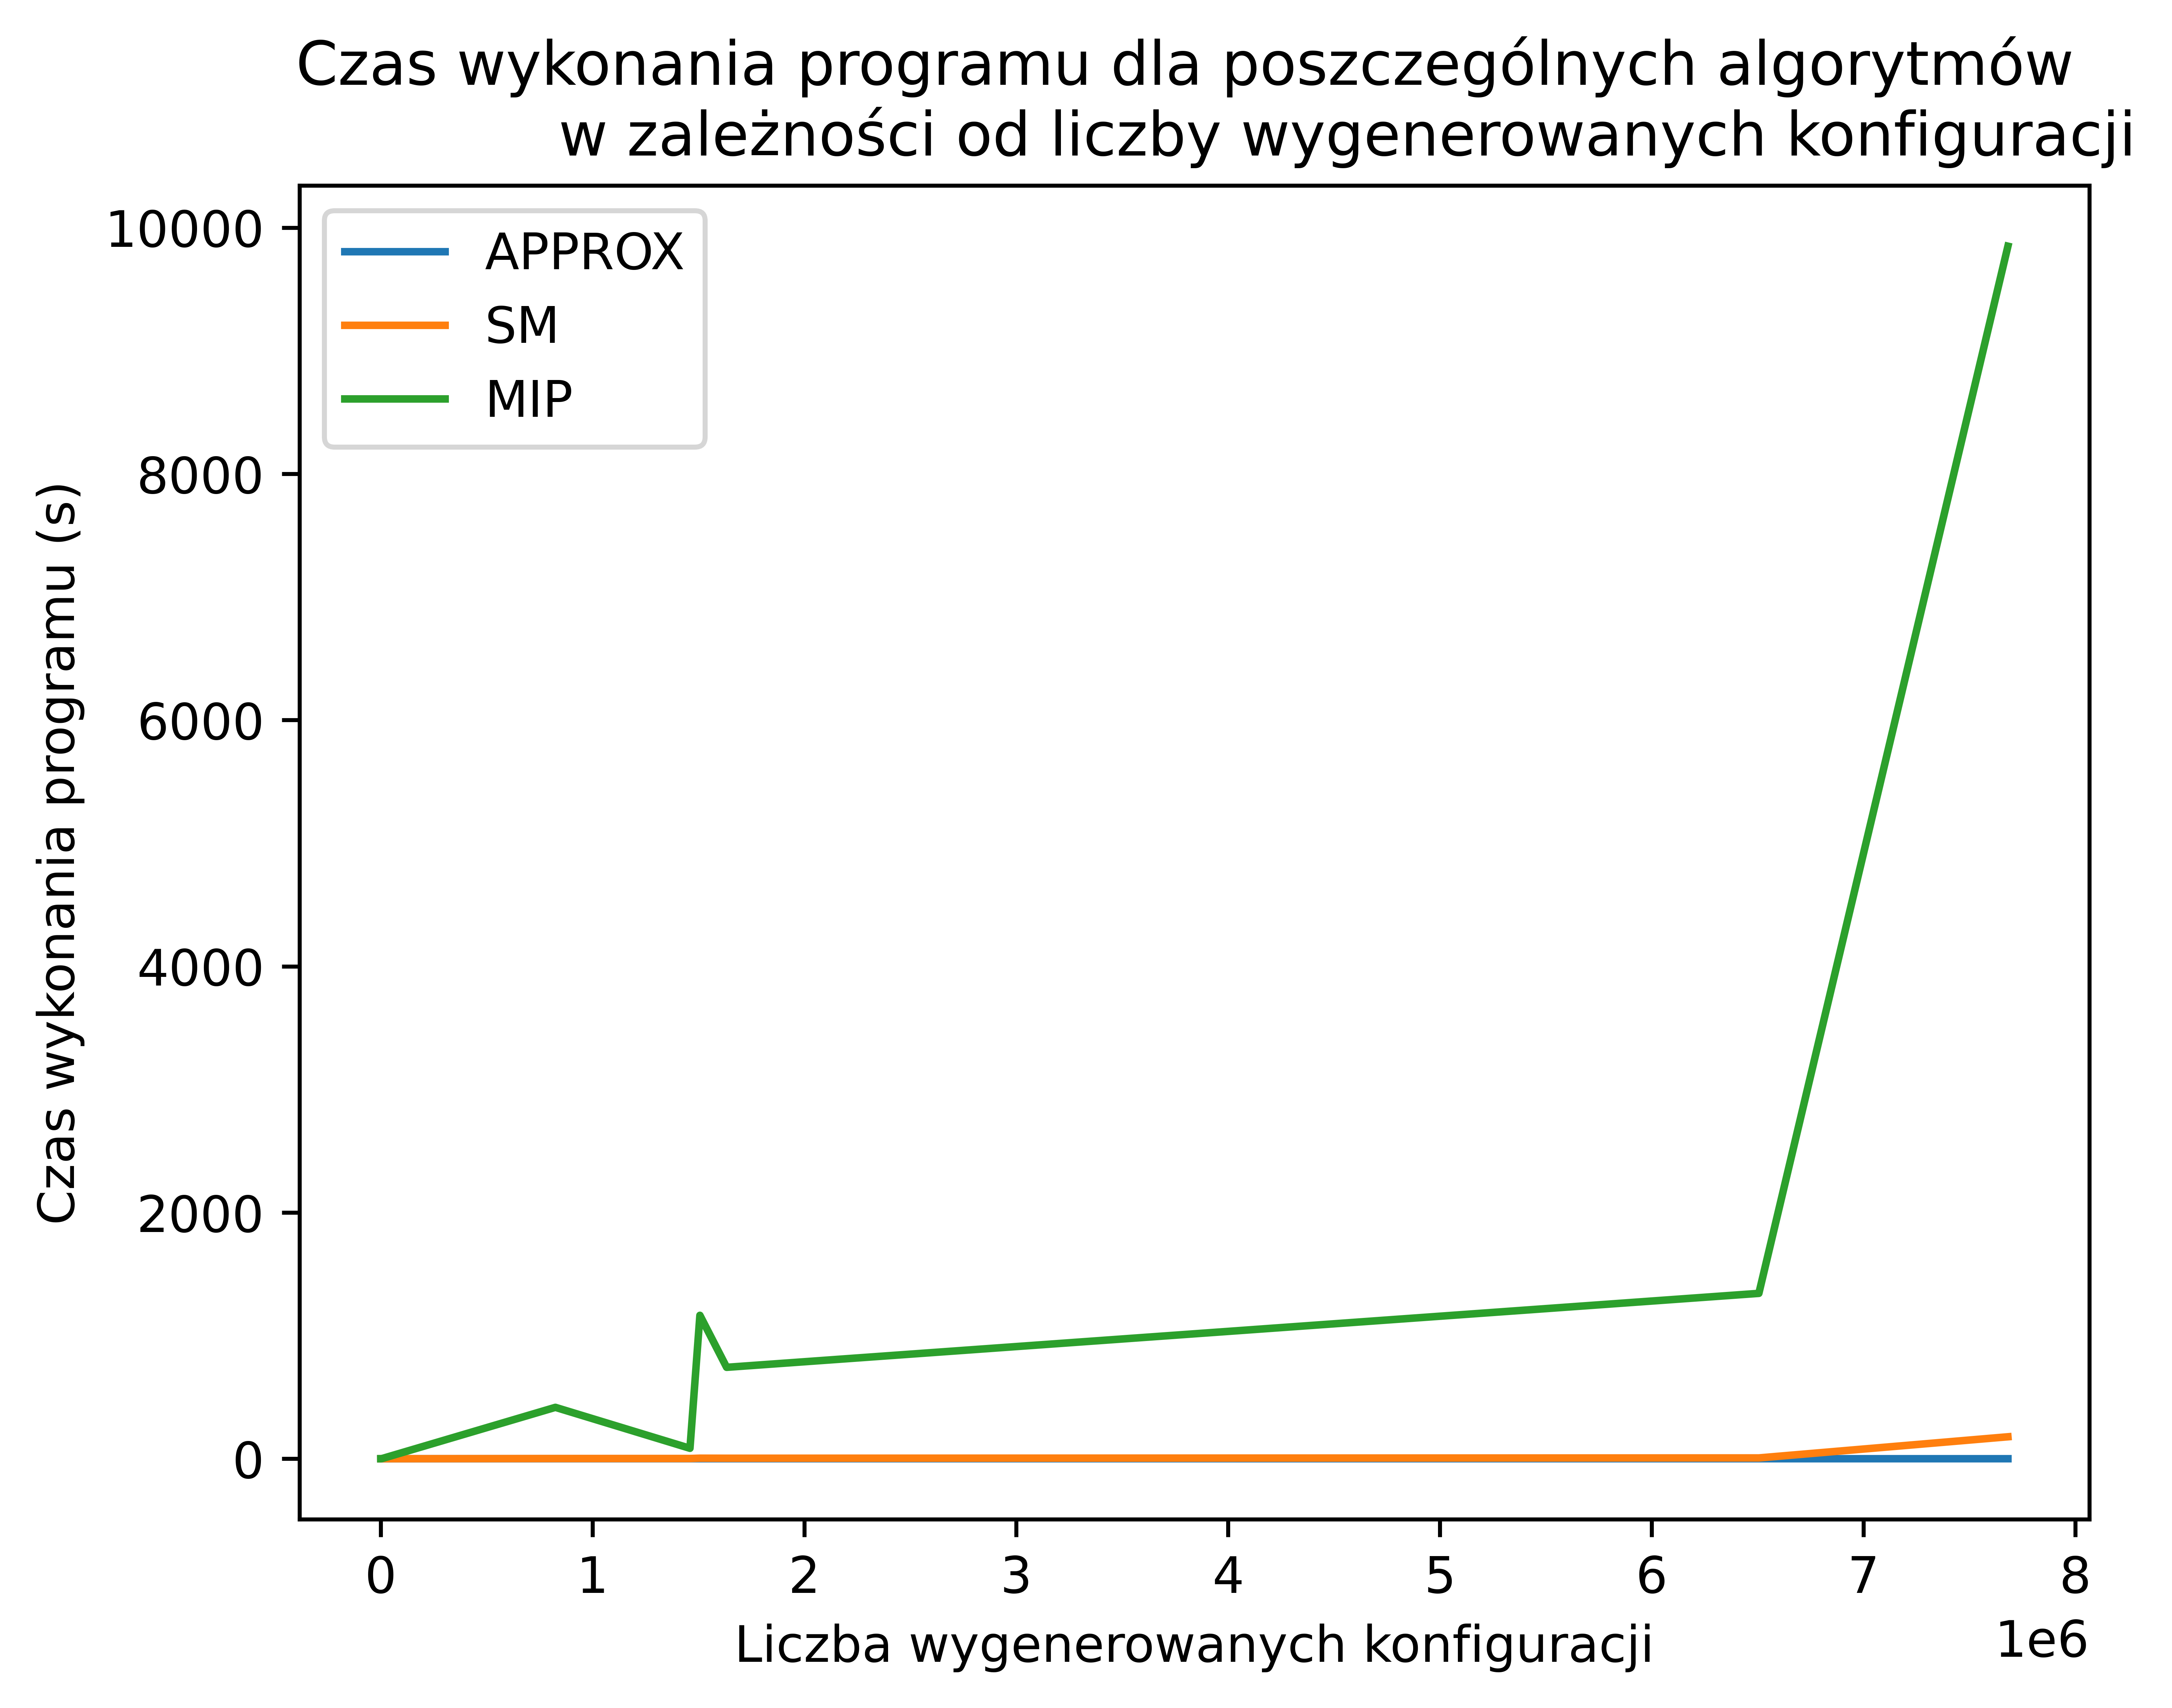
\includegraphics[width=12cm]{plots/time_configs}
		\caption{Wykres przedstawiający czas wykonania programu dla poszczególnych algorytmów w zależności od liczby wygenerowanych konfiguracji.}
	\end{center}
\end{figure}
%\fi

\newpage
\section{Obserwacje}

W powyższych danych można zauważyć, że
\begin{itemize}
	\item otrzymane rozwiązania są często blisko dolnej granicy:
	\begin{itemize}
		\item jest równe w pięciu, większe o jeden w trzech przypadkach dla APPROX \\
		Tylko w teście numer zero różnica ta wynosiła dziewięć belek na niekorzyść tej metody, co daje w przybliżeniu 112,32 procent kosztu rozwiązania optymalnego. Owa wartość mieści się w absolutnym współczynniku aproksymacji tego problemu: $3/2$, jednak wykracza poza średni wynoszący dla algorytmu FFD $11/9$.
		\item jest równe w siedmiu, większe o jeden w trzech przypadkach dla SM
		\item jest równe w dziewięciu przypadkach dla MIP
	\end{itemize}
	\item Algorytmy posiadają bardzo zróżnicowany czas działania.
	Program używający algorytmu aproksymacyjnego nie przekroczył nigdy dwóch milisekund, a najczęściej nawet jednej - stąd wartość zero w tabelach i wykresach. Natomiast MIP potrafił działać nawet prawie trzy godziny (test drugi - 9849.150s) zanim znalazł optymalne rozwiązanie. 
	\item Znaczący wpływ na liczbę możliwych konfiguracji ma duża liczba małych elementów.
	
\end{itemize}

\section{Wnioski}

\begin{itemize}
	\item Dla wielu instancji problemu cięcia belek może sie okazać, że rozwiązanie obliczone przy pomocy algorytmy aproksymacyjnego FFD będzie często bliskie rozwiązania optymalnego.
	\item W przypadku optymalizacji dyskretnej dużo czasu zajmuje znalezienie rozwiązania optymalnego pod kątem całkowitoliczbowym, w kontraście do szybkiego znajdowania optymalnego rozwiązania problemu pochodnego (poddanego relaksacji) algorytmem simpleks.
	\item Potwierdza się informacja dotycząca metody branch-and-cut zawarta w dokumentacji: \textit{GLPK branch-and-cut solver is not perfect, so it is unable to solve hard or very large scale MIP instances for a reasonable time.} Gdyby zwiększyć liczbę potrzebnych małych elementów do dwudziestu dla każdego rodzaju, program działałby dłużej niż najdłuższy zaprezentowany test (powyżej trzech godzin).
	\item Generowanie wszystkich możliwych konfiguracji i decydowanie o ich wyborze po fakcie ich wygenerowania nie sprawdzi się w przypadku maszyn z małą ilościa pamięci operacyjnej.
\end{itemize}







	\cleardoublepage
	
	\chapter{Podsumowanie} \label{ch:SUMMARY}
\addcontentsline{toc}{chapter}{Podsumowanie}
\thispagestyle{chapterBeginStyle}

W pracy przeanalizowano jednowymiarowy, optymalizacyjny Problem Cięcia Belek dla którego liczba typów elementów jest stała. 
Następnie przedstawiono cztery wybrane algorytmu rozwiązujące go. W programie dołączonym do pracy, którego szczegóły techniczne opisano, zaimplementowano trzy z nich. Na końcu przedstawiono wyniki testów, które miały na celu zbadanie optymalności zwracanych przez program rozwiązań.

\section{Wnioski}
Na podstawie przeglądu literatury, analizy badanego problemu, przeprowadzonych testów zostały wyciągnięte  przez autora pracy następujące wnioski:
\begin{enumerate}
	\item Często mogłoby się okazać, że nawet dla dużych instancji problemu algorytm aproksymacyjny zwróci optymalne bądź bliskie (np. optymalne plus jeden) takiemu rozwiązanie, w sytuacji gdy sprawdzić to można patrząc na ograniczenie dolne. Dlatego nawet gdyby autor dysponował implementacją algorytmu OPT+1, dla zaoszczędzenia czasu, uruchamiałby go jako drugi w kolejności, gdyby rozwiązanie zwrócone przez FFD byłoby dalekie od optymalnego.
	\item W powyższej sytuacji, w algorytmie OPT+1, zbiór na którym wykonywane jest przeszukiwanie binarne liczby belek, dla których problem jest spełnialny, mógłby początkowo być ograniczony z dołu przez obliczone ograniczenie dolne, a z góry przez liczbę potrzebnych belek otrzymanej przy pomocy algorytmu aproksymacyjnego.
	\item Z powodu gwałtownego wzrostu czasu spowodowanego dużą ilością ograniczeń całkowitoliczbowych dla danej instancji problemu, obiecująca wydaje się być część algorytmu OPT + 1, która nakłada owe ograniczenia tylko dla dużych konfiguracji, a małymi elementami zajmuje się po rozwiązaniu głównego MIP (wciaż bez ograniczeń na ich całkowitość).
	\item Jednak nawet gdyby pokuszono się o implementację algorytmu OPT+1, to przez fakt wykorzystanego w nim podejścia generowania wszystkich możliwych konfiguracji, dla ogromnych instancji problemów, obliczenia byłyby niewykonalne (głownie za sprawą dużej liczby zmiennych). Dla takich przypadków możnaby pochylić się nad metodą opisaną w pracy: \textit{A Linear Programming Approach to the Cutting-Stock Problem}\cite{GOMORY}.

\end{enumerate}

\section{Możliwe rozszerzenia pracy}
\begin{itemize}
	\item Modyfikacja obecnej wersji algorytmu MIP zgodnie z wnioskiem numer trzy.
	\item Zaimplementowanie algorytmu wspomnianego we wniosku numer cztery.
	\item Zamiana solvera GLPK na szybszy, np. CPLEX \cite{GLPK_BENCHMARK}.
	\item Przeprowadzenie bardziej szczegółowych testów obecnych jak i wspomnianych wyżej algorytmów na większej liczbie prób, badając przy tym więcej zależności takich jak np. wpływ stosunku małych elementów do dużych na czas wykonania programu, liczbę konfiguracji.
\end{itemize}



	\cleardoublepage
	
	
	%%%%%%%%%%%%%%%%%%%%%%%%%%%%%%%%%%%%%%%%%%%%%%%%%%%%%%%%%%%%%%%%%%%%%%%%%%%%%%
	%%%%%%%%%%%%%%%%%%%%%%%%%%%%%%% BIBLIOGRAFIA %%%%%%%%%%%%%%%%%%%%%%%%%%%%%%%%%
	%%%%%%%%%%%%%%%%%%%%%%%%%%%%%%%%%%%%%%%%%%%%%%%%%%%%%%%%%%%%%%%%%%%%%%%%%%%%%%

	\pagestyle{bibliographyStyle}
	\bibliographystyle{plabbrv}
	\bibliography{literatura}
	\thispagestyle{chapterBeginStyle}
        \addcontentsline{toc}{chapter}{Bibliografia}
	\cleardoublepage
	
	%%%%%%%%%%%%%%%%%%%%%%%%%%%%%%%%%%%%%%%%%%%%%%%%%%%%%%%%%%%%%%%%%%%%%%%%%%%%%%
	%%%%%%%%%%%%%%%%%%%%%%%%%%%%%%%%% DODATKI %%%%%%%%%%%%%%%%%%%%%%%%%%%%%%%%%%%%
	%%%%%%%%%%%%%%%%%%%%%%%%%%%%%%%%%%%%%%%%%%%%%%%%%%%%%%%%%%%%%%%%%%%%%%%%%%%%%%
	
	\appendix
	\pagestyle{appendixStyle}
       \renewcommand{\appendixname}{Załącznik}
	
	\chapter{Zawartość płyty CD}
\thispagestyle{chapterBeginStyle}
\label{plytaCD}

Na płycie CD dołączonej do niniejszej pracy znajdują się:
\begin{enumerate}
	\item Kody źródłowe (katalog \verb|PDF|) w języku LATEX teoretycznej części pracy wraz z niezbędnymi grafikami.
    \item Plik PDF (\verb|PDF/praca.pdf|) - wynik kompilacji plików z punktu 1.
	\item Kody źródłowe części praktycznej (katalog \verb|SourceCode|) w języku C, bash, Python. Struktura projektu prezentuje się następująco:
	
	\dirtree{%
		.1 SourceCode.
		.2 Makefile.
		.2 bin.
		.3 main.
		.2 obj.
		.2 src.
		.3 approx.c.
		.3 approx.h.
		.3 gen\_configs.c.
		.3 io\_handler.c.
		.3 io\_handler.h.
		.3 main.c.
		.3 solver\_part.c.
		.3 solver\_part.h.
		.3 structs.h.
		.3 vector.c.
		.3 vector.h.
		.1 Tests.
		.2 input.
		.2 ouput.
		.2 solver\_logs.
		.2 run\_tests.sh.
		.2 generate\_plots.py.
		.2 latex\_table.py.
	}
\end{enumerate}




	
	\cleardoublepage

\end{document}

